%%%%%%%%%%%%%%%%%%%%%%%%%%%%%%%%%%%%%%%%%%%%%%%%%%%%%%%%%%%%%%%%%%%%%%%%%%%%%%%%%%%%%%%%%%%%%%%%%%%%%%%%%%%%%%%%%%%%%%%%%%%%%%%%%%%%%%%%%%%%%%%%%%%%%%%%%%%%%%%%%%%%%%%%%%%%%%%%%%%%%%%%%%%%%%%%%%%%%%%%%%%%%%%%%%%%%%%%%%%%%%%%%%%
%%%%%%%%%%%%%%%%%%%%%%%%%%%%%%%%%%%%%%%%%%%%%%%%%%%%%%%%%%%%%%%%%%%%%%%%%%%%%%%%%%%%%%%%%%%%%%%%%%%%%%%%%%%%%%%%%%%%%%%%%%%%%%%%%%%%%%%%%%%%%%%%%%%%%%%%%%%%%%%%%%%%%%%%%%%%%%%%%%%%%%%%%%%%%%%%%%%%%%%%%%%%%%%%%%%%%%%%%%%%%%%%%%%
%%%%%%%%%%%%%%%%%%%%%%%%%%%%%%%%%%%%%%%%%%%%%%%%%%%%%%%%%%%%%%%%%%%%%%%%%%%%%%%%%%%%%%%%%%%%%%%%%%%%%%%%%%%%%%%%%%%%%%%%%%%%%%%%%%%%%%%%%%%%%%%%%%%%%%%%%%%%%%%%%%%%%%%%%%%%%%%%%%%%%%%%%%%%%%%%%%%%%%%%%%%%%%%%%%%%%%%%%%%%%%%%%%%
\chapter{The Large Hadron Collider}

The Large Hadron Collider (LHC)~\cite{bib:LHC_machine_2008,bib:LHC_2004} is a particle accelerator installed in the former LEP~\cite{bib:LEP_design_1984} tunnel at CERN\footnote{European Organisation for Nuclear Research}.
It is 26.7\km in circumference and consists of two separate rings, which are, in periods of operation, inhabited by two counter-circulating beams.
At the interaction points of the two beams, either proton-proton collisions or heavy ion collisions take place.
In this thesis, only \pp-collision data from the year 2012 is analysed.
Thus, all machine values cited in the following chapters and paragraphs refer to the setup for $pp$~collisions in 2012 if not stated otherwise.

The beams are separated into bunches which rotate with a bunch spacing of 50\ns corresponding to a collision frequency of 20\mhz.
Before the bunches are actually filled into the LHC ring they are pre-accelerated in other accelerators, which are in the order they are actually passed by the protons: Linac2, Proton  Synchrotron Booster (PSB), Proton Synchrotron (PS), Super Proton Synchrotron (SPS).
The beam energy is 450\gev when the beams enter the LHC ring.
The injector chain and the LHC ring with its experiments are visualised in Fig~\ref{fig:LHC}.
\begin{figure}[!b]
  \centering
      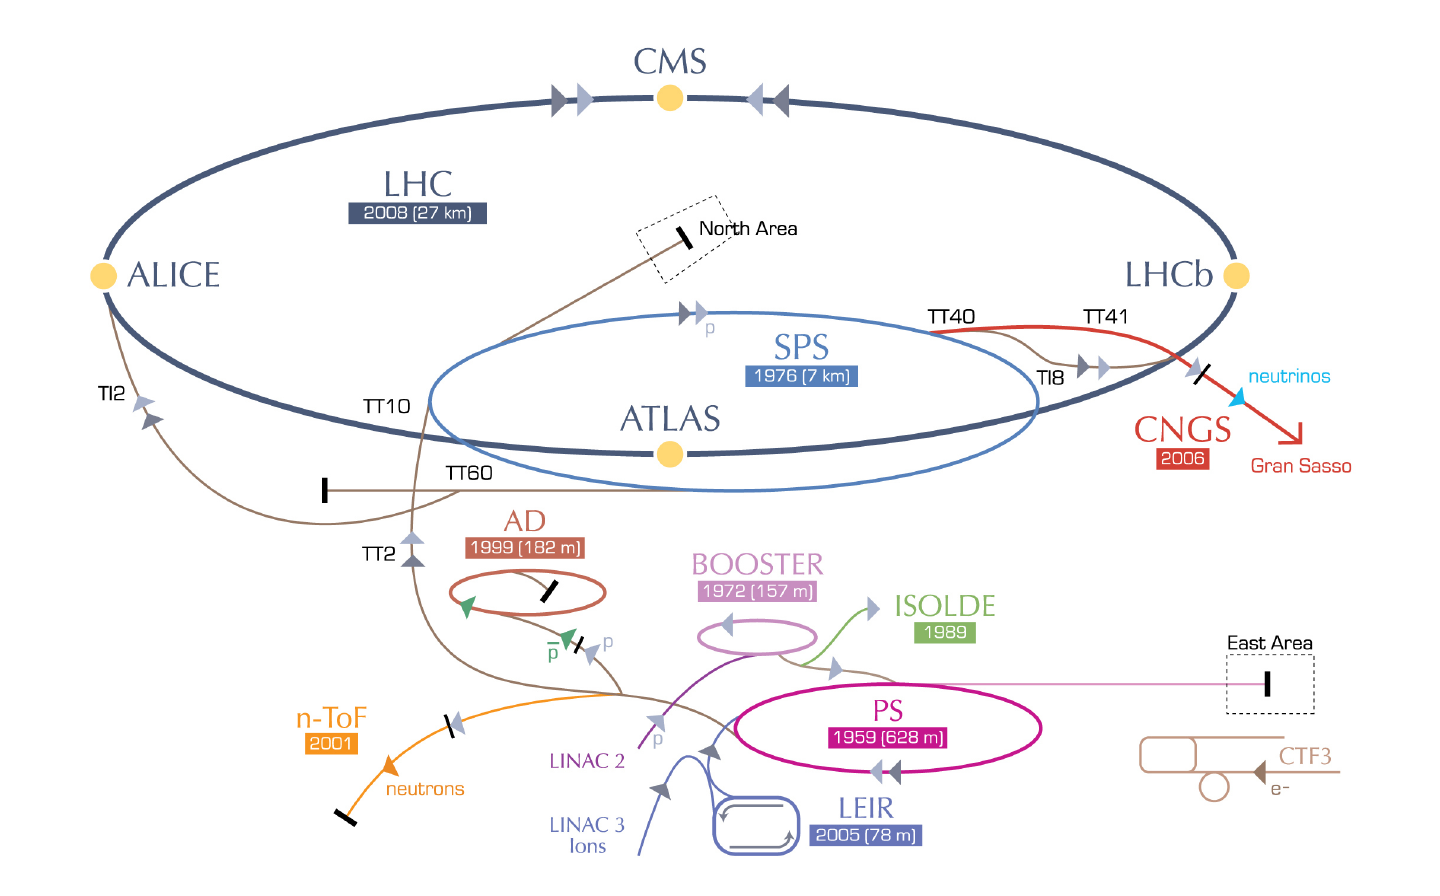
\includegraphics[width=0.83\textwidth]{figures/experiment/LHC/LHC_small.png}
  \caption{Visualisation of the LHC with its experiments and the injector chain. Taken from~\cite{bib:CERNBrochure}.}  
  \label{fig:LHC}
\end{figure}

In the LHC, the beams are kept on their circular path with the help of a magnetic dipole field of 4.76\tesla.
Further quadrupole and sextupole magnets squeeze and focus the bunches resulting in a bunch spread of roughly 8\cm length and a Gaussian shape radius of 20\mum RMS at the interaction point.
The number of protons contained in each bunch is of the order $10^{11}$.
The LHC hosts four main particle physics experiments: the CMS, ATLAS, LHCb and ALICE experiments.
CMS~\cite{bib:CMS:experiment,bib:CMS:TDR} and ATLAS~\cite{bib:ATLAS:experiment,bib:ATLAS:TDR_1,bib:ATLAS:TDR_2} are so-called ``general purpose experiments'', that are used for a variety of different physics analyses.
In contrast, the LHCb~\cite{bib:LHCb:experiment} and ALICE~\cite{bib:ALICE:experiment} experiments are designed with an emphasis on CP-violation measurements and heavy ion collisions, respectively.

The number of expected events $N$ for a given process can be expressed in terms of the corresponding cross section $\sigma$ times the integrated luminosity $L$
\begin{equation}
N = L \cdot \sigma,
\end{equation}
with an integrated luminosity of $L=\int \mathcal{L}\, dt$, where $\mathcal{L}$ is the instantaneous luminosity.
The instantaneous luminosity $\mathcal{L}$ depends on several machine parameters, such as the collision frequency $f$, the number of particles in the bunches $n_1$ and $n_2$,
the spread in the transverse plane of the bunches $\sigma_x$ and $\sigma_y$, and a geometrical correction parameter $F$ due to the crossing angle of the two bunches at the interaction point:
\begin{equation}
\mathcal{L} = \frac{f n_1 n_2 }{4 \pi \sigma_x \sigma_y} \cdot F.
\end{equation}
In 2012, the peak luminosity was $7.7 \cdot 10^{33} \frac{1}{\text{cm}^2\,\text{s}}$.
The total integrated luminosity of $pp$~collisions over time recorded at the CMS experiment is shown in Fig.~\ref{fig:Lumi}.
\begin{figure}[!b]
  \centering
      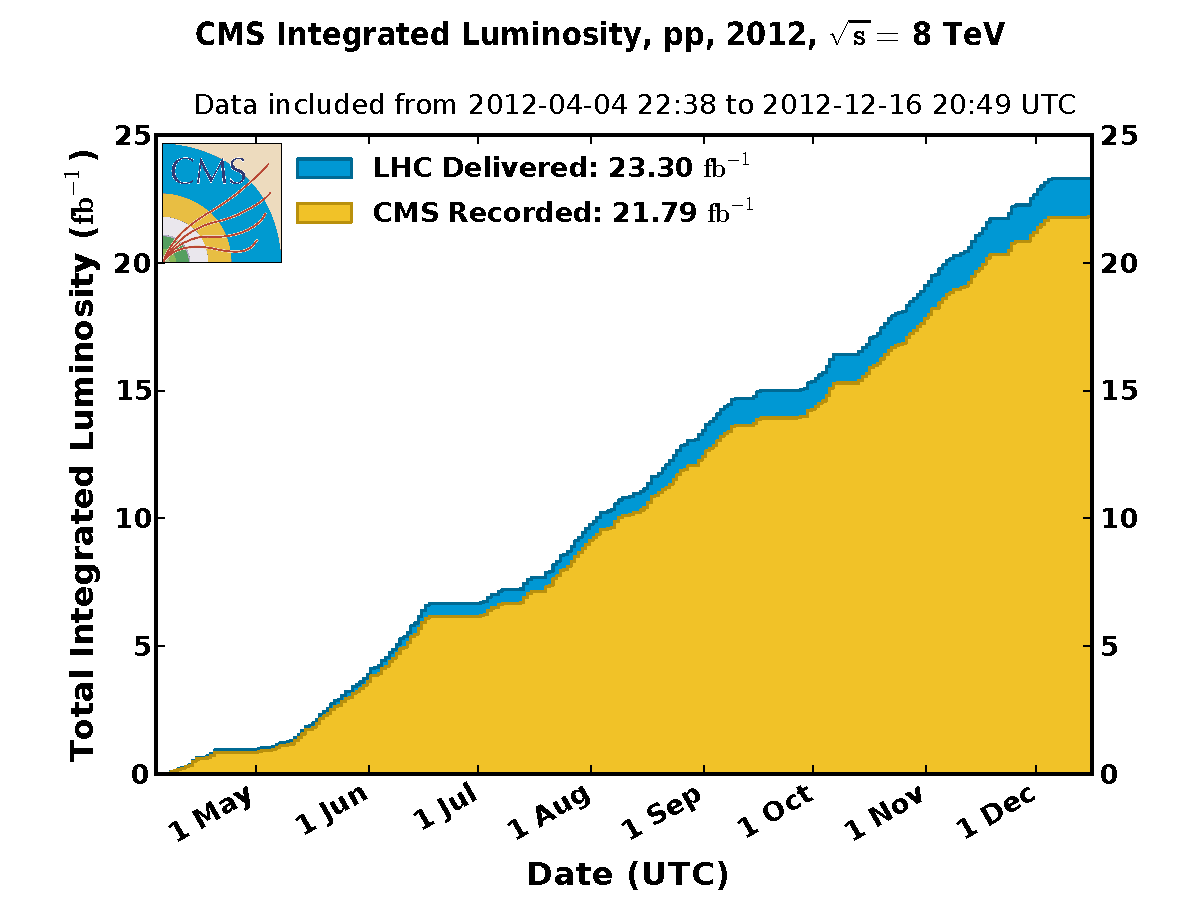
\includegraphics[width=0.57\textwidth]{figures/experiment/LHC/int_lumi_per_day_cumulative_pp_2012.pdf}
  \caption{Integrated luminosity delivered by LHC (blue) and recorded by CMS (orange) in the year 2012. Taken from~\cite{bib:LumiWiki}.}  
  \label{fig:Lumi}
\end{figure}
Events recorded at the CMS experiment are grouped together within ``luminosity blocks''.
They refer to short intervals of data taking ($\sim$2-3\,min) in which the instantaneous luminosity is stable.
In addition, luminosity blocks are comprised to so-called ``runs''.
They correspond to periods of data taking over which the overall conditions remain almost stable.
%%%%%%%%%%%%%%%%%%%%%%%%%%%%%%%%%%%%%%%%%%%%%%%%%%%%%%%%%%%%%%%%%%%%%%%%%%%%%%%%%%%%%%%%%%%%%%%%%%%%%%%%%%%%%%%%%%%%%%%%%%%%%%%%%%%%%%%%%%%%%%%%%%%%%%%%%%%%%%%%%%%%%%%%%%%%%%%%%%%%%%%%%%%%%%%%%%%%%%%%%%%%%%%%%%%%%%%%%%%%%%%%%%%
%%%%%%%%%%%%%%%%%%%%%%%%%%%%%%%%%%%%%%%%%%%%%%%%%%%%%%%%%%%%%%%%%%%%%%%%%%%%%%%%%%%%%%%%%%%%%%%%%%%%%%%%%%%%%%%%%%%%%%%%%%%%%%%%%%%%%%%%%%%%%%%%%%%%%%%%%%%%%%%%%%%%%%%%%%%%%%%%%%%%%%%%%%%%%%%%%%%%%%%%%%%%%%%%%%%%%%%%%%%%%%%%%%%
%%%%%%%%%%%%%%%%%%%%%%%%%%%%%%%%%%%%%%%%%%%%%%%%%%%%%%%%%%%%%%%%%%%%%%%%%%%%%%%%%%%%%%%%%%%%%%%%%%%%%%%%%%%%%%%%%%%%%%%%%%%%%%%%%%%%%%%%%%%%%%%%%%%%%%%%%%%%%%%%%%%%%%%%%%%%%%%%%%%%%%%%%%%%%%%%%%%%%%%%%%%%%%%%%%%%%%%%%%%%%%%%%%%
\FloatBarrier
\chapter{The CMS detector}
The Compact Muon Solenoid (CMS) detector~\cite{bib:CMS:experiment,bib:CMS:TDR} is a general purpose detector, designed to explore particle physics phenomena up to the multi-TeV scale.
The detector concept is an onion-like structure of different layers, each one made up of a different type of detector. 
The CMS detector measures 21.6\m in length and 14.6\m in diameter with a total weight of 12\,500\,tons.
In Fig.~\ref{fig:CMSdetector}, a perspective view of the CMS detector is depicted. 
\begin{figure}[!b]
  \centering
      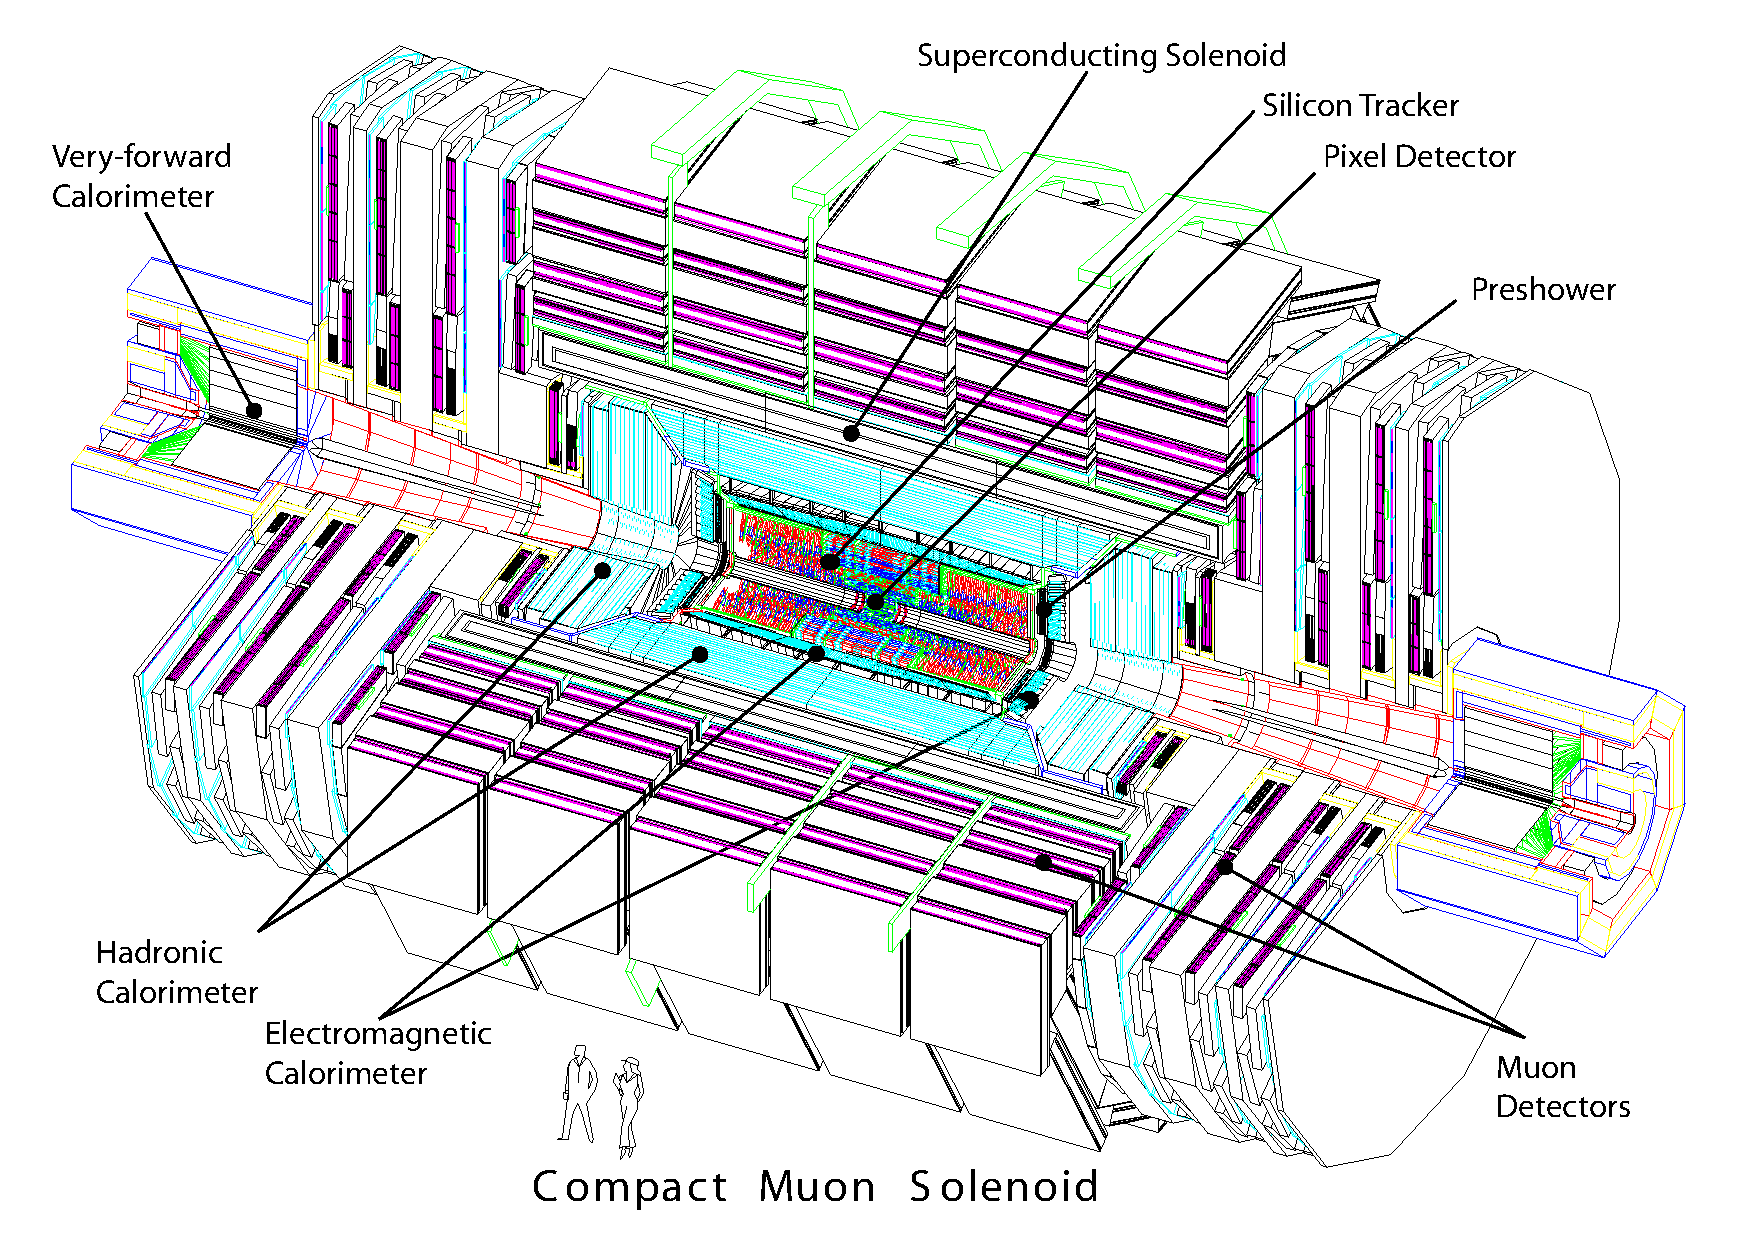
\includegraphics[width=0.84\textwidth]{figures/experiment/CMS/cms_complete_labelled_reduced_size.pdf}
  \caption{A perspective view of the CMS detector. Taken from~\cite{bib:CMS:experiment}}  
  \label{fig:CMSdetector}
\end{figure}

The coordinate system used at CMS consists of the pseudorapidity $\eta = -\ln \left[ \tan{\left(\theta/2\right)} \right]$ and the azimuthal angle $\phi$.
The advantage of the pseudorapidity $\eta$ is the Lorentz invariance with respect to the z-axis (beam axis).
The angle $\phi$ covers the direction in the $x-y$ plane (orthogonal to the beam axis).
Since the CMS experiment utilises proton-proton collisions, where the inelastic scattering happens on parton level, the initial total momentum of the corresponding partons are unknown.
Thus, instead of exploiting the conservation of total momentum, only the conservation of transverse momentum is usually used.
This can be done because the partons have no (or only an negligible amount) of initial momentum in the transverse plane.
Thus the initial state is characterised by $\sum{\pt}=0$, with $\pt = \sqrt{p_x^2 + p_y^2}$.

In order to bend the particle trajectories and thus to measure the momentum of charged particles a superconducting solenoid is incorporated between the calorimeter system and the muon system (see Fig.~\ref{fig:CMSdetector}) providing a uniform axial magnet field of 3.8\tesla.
Iron yokes contained within the muon system ensure the return of the magnetic flux. 

In the following, the various detector components of the CMS detector from the inside to the outside as well as the trigger system will be explained.
%%%%%%%%%%%%%%%%%%%%%%%%%%%%%%%%%%%%%%%%%%%%%%%%%%%%%%%%%%%%%%%%%%%%%%%%%%%%%%%%%%%%%%%%%%%%%%%%%%%%%%%%%%%%%%%%%%%%%%%%%%%%%%%%%%%%%%%%%%%%%%%%%%%%%%%%%%%%%%%%%%%%%%%%%%%%%%%%%%%%%%%%%%%%%%%%%%%%%%%%%%%%%%%%%%%%%%%%%%%%%%%%%%%
\FloatBarrier
\section{The tracking system}
\label{sec:TrackingSystem}
The tracking detector~\cite{bib:CMS:TDR_2006,bib:CMS:Tracker_1997,bib:CMS:Tracker_2000} is the innermost detector at CMS. 
It is a silicon semiconductor detector and is included for the tasks of vertex and track reconstruction by the measurement of particles' energy losses.
A schematic sketch of the tracker at CMS is depicted in Fig.~\ref{fig:Tracker}.
\begin{figure}[!b]
  \centering
      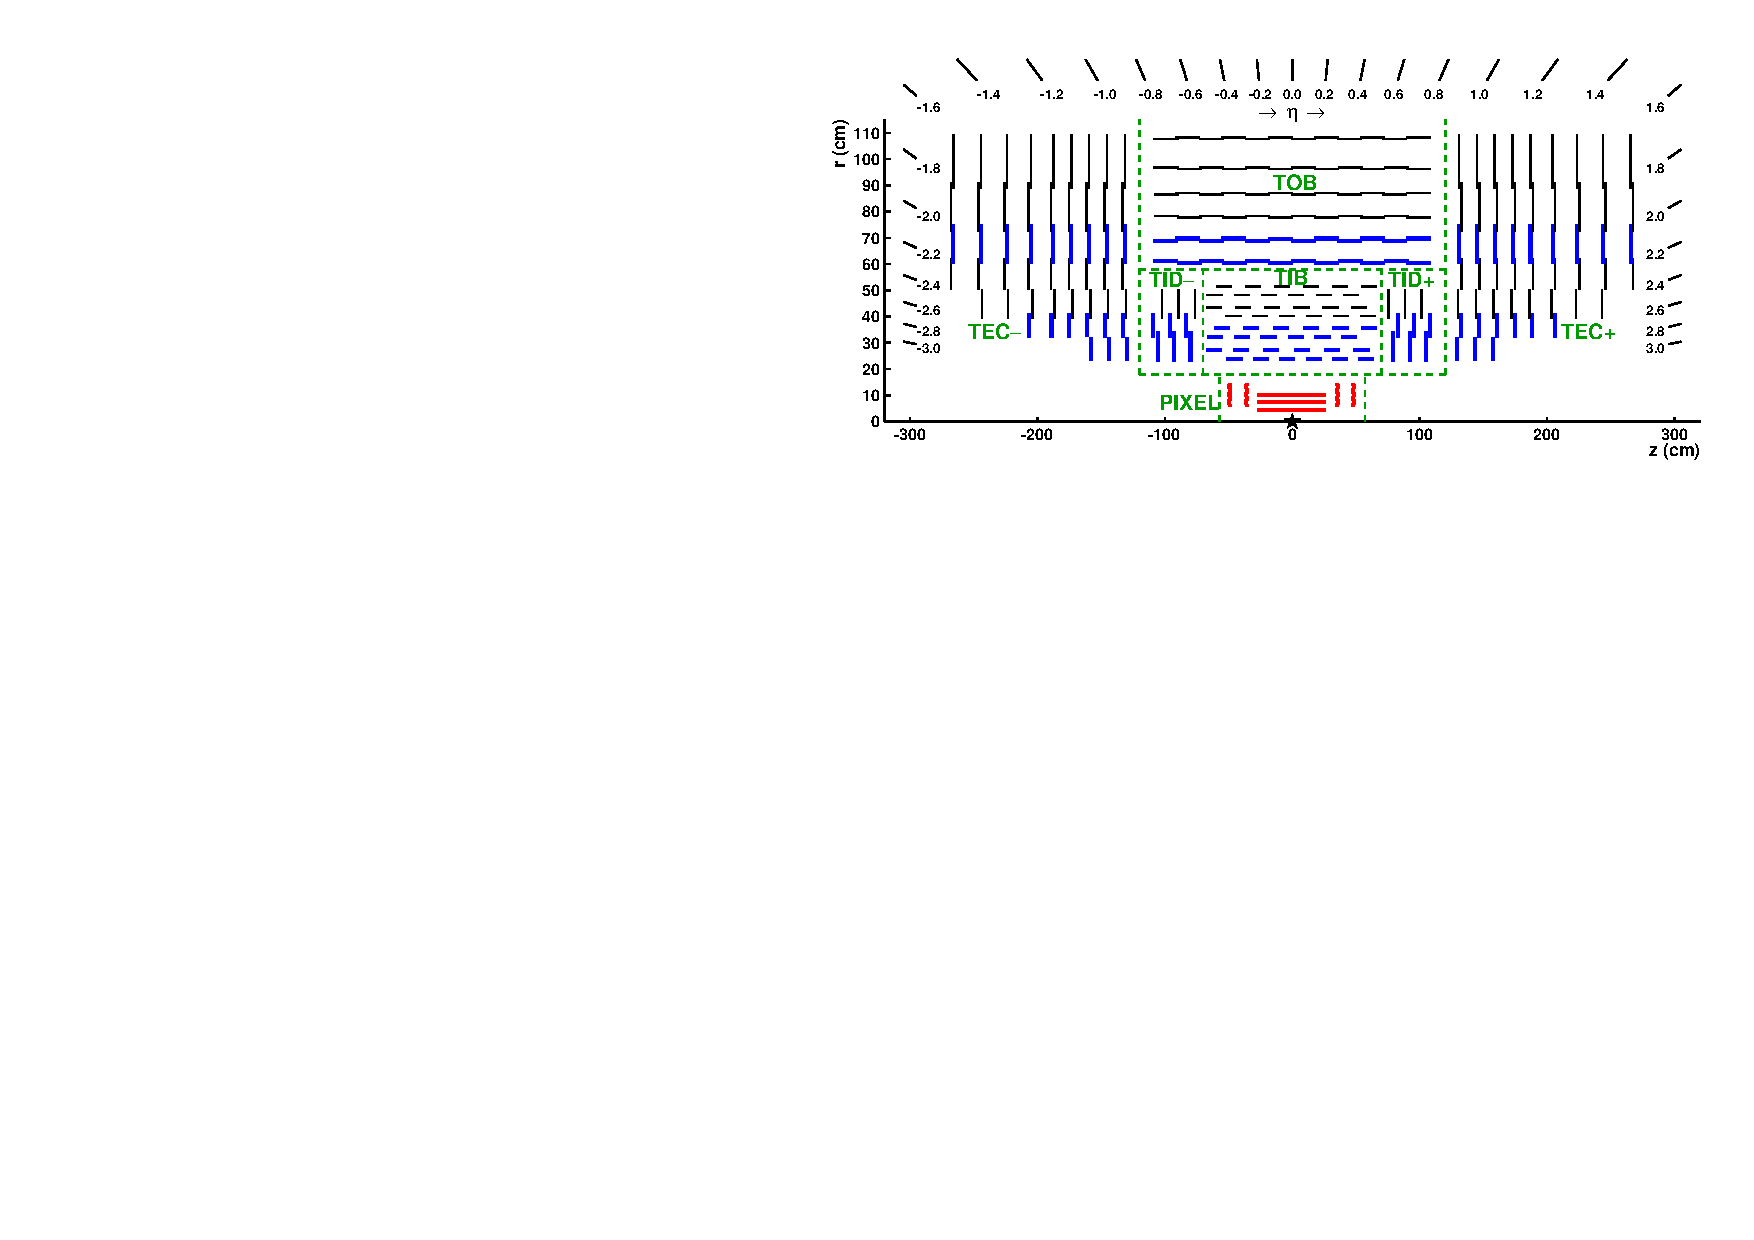
\includegraphics[width=0.95\textwidth]{figures/experiment/CMS/TrackerLayoutNew.pdf}
  \caption{Schematic sketch of the silicon tracker at CMS in the $r - z$ plane including the silicon pixel detector (PIXEL) as well as the different components of the silicon strip detector: tracker inner barrel (TIB), tracker outer barrel (TOB), tracker endcap (TEC), and tracker inner disk (TID). Taken from~\cite{bib:CMS:tracking_8TeV}.
           }  
  \label{fig:Tracker}
\end{figure}
The tracking system is divided into two parts: the innermost tracker is a silicon pixel detector surrounded by a silicon strip detector.
Since the silicon pixel tracker is closest to the interaction point and has thus to deal with much higher particle fluxes, its granularity is higher compared to the silicon strip detector.

Both parts will be explained in detail in the upcoming sections.
Because, the variable \dedx, the energy loss per path length, is used in this thesis for the search for highly ionising, short tracks (Part~\ref{part:analysis}), the last part of this section is dedicated to a short description of how the energy of a traversing particle is measured with the silicon sensors.
Furthermore, since a calibration of the silicon pixel detector was performed within this PhD thesis (see Section~\ref{sec:EnergyCalibration}), an emphasis will be put on the pixel detector.

%%%%%%%%%%%%%%%%%%%%%%%%%%%%%%%%%%%%%%%%%%%%%%%%%%%%%%%%%%%%%%%%%%%%%%%%%%%%%%%%%%%%%%%%%%%%%%%%%%%%%%%%%%%%%%%%%%%%%%%%%%%%%%%%%%%%%%%%%%%%%%%%%%%%%%%%%%%%%%%%%%%%%%%%%%%%%%%%%%%%%%%%%%%%%%%%%%%%%%%%%%%%%%%%%%%%%%%%%%%%%%%%%%%
\subsection*{The silicon pixel tracker}
The silicon pixel detector consists of three different cylindrical layers in the barrel region at radii of 4.4\cm, 7.3\cm and 10.2\cm and two discs in the endcaps at $z$-distances of 34.5\cm and 46.5\cm.
It is made up of 1440 modules in total (barrel + endcaps), each module comprising 8 or 16 read-out-chips (ROCs).
The read-out-chips are bump bonded~\cite{Thesis_Jenny} to a pixel system of $52\times80$ pixels, which are read out in double columns (see~\cite{Thesis_Jenny} on detailed information of the readout electronics).
A visualisation of a part of a pixel module is shown in Fig.~\ref{fig:PixelTracker}.
\begin{figure}[!b]
  \centering
      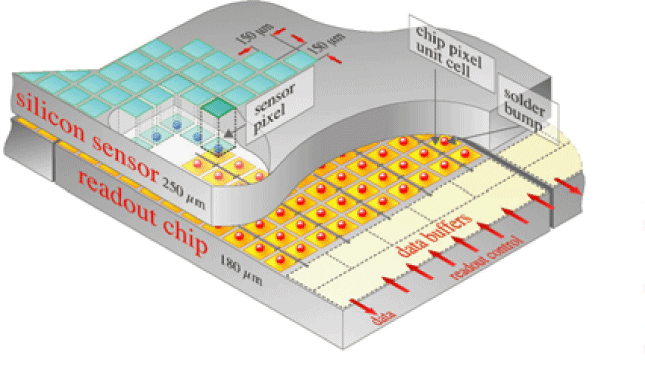
\includegraphics[width=0.60\textwidth]{figures/experiment/CMS/Pixelement.png}
  \caption{Schematic sketch of a part of a silicon pixel tracker module including the silicon sensors and the read-out-chip (ROC). Taken from~\cite{bib:PixelModule}.}  
  \label{fig:PixelTracker}
\end{figure}
In total, there are 65 million pixels comprised in the pixel detector.
The large number of pixels and their small size ensure a low occupancy close to the vertex of around $0.002 - 0.02$\%~\cite{bib:CMS:tracking_8TeV} and a high hit efficiency of around 99\%~\cite{bib:CMS:PixelSpatialResolution}. 

The silicon pixel detector is very important for the reconstruction of primary and secondary vertices as well as the reconstruction of particle tracks.
Therefore, a high spatial resolution is needed.
This is achieved by the small size of the pixels ($ 150 \times 100 \mum^2$) and the exploitation of the spread of the energy deposition across several pixels, called charge sharing (in average the energy is deposited across 3-5 pixels~\cite{bib:TWIKI:PixelClusterSize}).
Exploiting the energy spread across pixels, a spatial resolution in the barrel region of 9.4\mum in the $r - \phi$ plane and - dependent on the incident angle of a track - a hit resolution between $20-45\mum$ in the z-direction is achieved~\cite{bib:CMS:tracking_8TeV}. 
%The high spatial resolution makes the pixel detector perfectly suited for the reconstruction of vertices and tracks.
The spatial resolution of the primary vertex depends on the number of tracks taken into account for the reconstruction of the primary vertex.
For more than 50 tracks originating from the primary vertex the spatial resolution is around $10-12\mum$ for each of the three spatial dimensions~\cite{bib:CMS:tracking_8TeV}.
The reconstruction efficiency of primary vertices is close to 100\% if more than two tracks are used for the vertex reconstruction~\cite{bib:CMS:tracking_8TeV}.

\subsection*{The silicon strip tracker}
The silicon strip tracker is the next-to innermost detector of the CMS detector and ranges up to a radius of 1.1\m.
The barrel region consists of a tracker inner barrel (TIB) and a tracker outer barrel (TOB).
The TIB has four layers with two layers equipped with so-called ``stereo'' modules that can measure the hit position additionally in the $r-z$ plane.
The silicon sensors in the TIB are of 320\mum thickness with a strip pitch varying between $80-120\mum$.
The TOB has six different layers (two layers of stereo modules) with silicon sensors of 500\mum thickness and strip pitches between 120 and 180\mum. 

The endcaps are subdivided into a tracker endcap (TEC) and a tracker inner disk (TID).
They ensure a coverage of a pseudorapidity up to $|\eta|=2.5$.
In each TEC, 9 disks between a z-position of $120\cm < z < 280\cm$ are contained.
Each of the TID comprises three disks between $60\cm < z < 110\cm$.

In the barrel region, a single-point resolution between $23 - 52\mum$ in the $r-\phi$ plane and $230 - 530\mum$  in the z-direction is achieved.
%FIXME: What about momentum resolution

\subsection*{Energy measurements in the tracking system}
A charged particle traversing the above mentioned silicon detectors produces electron-hole pairs in the semiconducting material along its trajectory, thus loosing energy due to ionisation.
For silicon, the mean energy to create an electron-hole pair is 3.61\ev at $-10\degree$C.
Minimally ionising particles produce an average of 22\,000 electron-hole pairs in silicon sensors~\cite{Thesis_Jenny}.
Electrons that are subject to a hard collision with the incoming particle (so-called delta-rays), produce further ionisation and can thus lead to much higher energy deposits in the silicon.
Because of the applied bias voltage at the sensors (for the creation of a depletion zone), the released electrons (holes) travel to the n-contacts (p-contacts), thereby inducing a current proportional the released energy, which is measured by the readout electronics. 
A more detailed description of the energy measurement in silicon sensors can be found in~\cite{Thesis_Jenny}.

%%%%%%%%%%%%%%%%%%%%%%%%%%%%%%%%%%%%%%%%%%%%%%%%%%%%%%%%%%%%%%%%%%%%%%%%%%%%%%%%%%%%%%%%%%%%%%%%%%%%%%%%%%%%%%%%%%%%%%%%%%%%%%%%%%%%%%%%%%%%%%%%%%%%%%%%%%%%%%%%%%%%%%%%%%%%%%%%%%%%%%%%%%%%%%%%%%%%%%%%%%%%%%%%%%%%%%%%%%%%%%%%%%%
\section{The electromagnetic calorimeter}
The electromagnetic calorimeter (ECAL)~\cite{bib:CMS:TDR_2006,bib:CMS:TDR_ECAL} encloses the tracking system and starts at a radius of 129\cm in the barrel region.
It measures the energy and position of a traversing particle.
It is divided into a barrel part and two endcaps, which are at a distance of 314\cm from the vertex.
Figure~\ref{fig:ECAL} depicts a schematic sketch of the electromagnetic calorimeter system in the transverse plane.
\begin{figure}[!t]
  \centering
      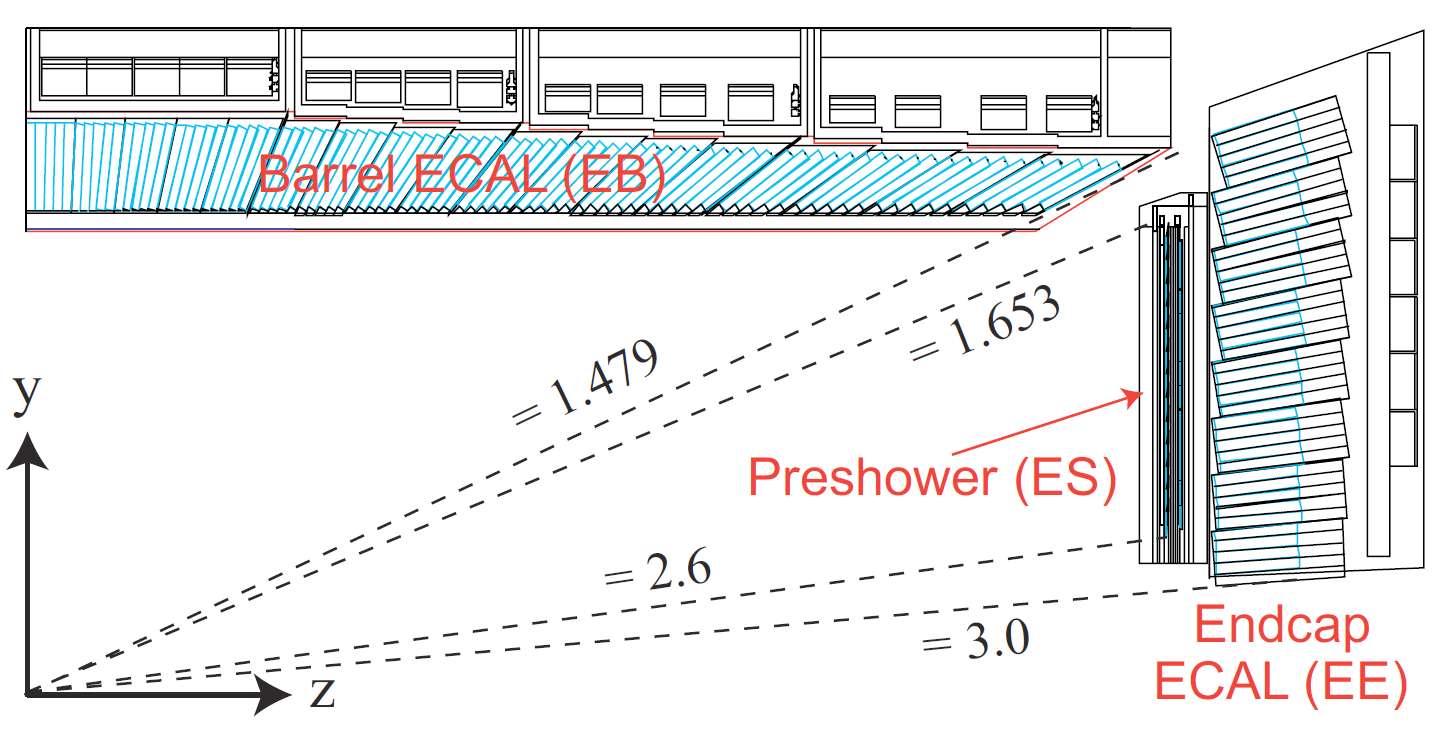
\includegraphics[width=0.65\textwidth]{figures/experiment/CMS/Figures_Experimental_Apparatus_ECALRapidity.png}
  \caption{A quarter section of the ECAL in the $r-z$ plane. Taken from~\cite{bib:CMS:TDR_2006}.}  
  \label{fig:ECAL}
\end{figure}
It can be seen, that the ECAL barrel~(EB) covers a pseudorapidity region up to $|\eta|=1.479$.
The ECAL endcaps~(EE) start at $|\eta|=1.653$ and reach up to $|\eta|=3.0$.
In front of the endcaps, a preshower detector ($1.653<|\eta|<2.6$) is installed with the main task to identify neutral pions.
It additionally improves the position measurement of electrons and photons.

The EB and EE consist of lead tungstate (PbWO$_4$) scintillating crystals, 61200 in the barrel region and 7324 in each of the endcaps. 
Their advantage is the short radiation length ($X_0=0.89\cm$) and a small Moli\`ere radius (2.2\cm).
Thus, particles deposit their energy on rather short distances and a compact design is possible.
Since they lack a fine longitudinal segmentation, the information on the shower development is limited.
To detect the rather low light yield ($30\,\gamma/\mev$) of a traversing particle, silicon avalanche photodiodes (APDs) are used in the barrel region and vacuum  phototriodes (VPTs) in the endcaps.
For information on the readout electronics, the reader is referred to~\cite{bib:CMS:TDR_2006}.

The resolution of an energy measurement in the calorimeter can be expressed by 
\begin{equation}
\label{eq:CaloResolution}
\left( \frac{\sigma}{E} \right)^2 = \left( \frac{S}{\sqrt{E}} \right)^2 + \left( \frac{N}{E} \right)^2 +C^2,
\end{equation}
with $S$ referring to the stochastic term, $N$ to the noise term, and $C$ to a constant term.
For the ECAL at CMS the parameters of Eq.~\eqref{eq:CaloResolution} are measured to $S=3.63\,\sqrt{\text{GeV}}$, $N=0.124\gev$, and $C=0.26$~\cite{bib:CMS:TDR_2006}. 
These numbers lead to an energy resolution of around 0.4\% for an electron with $E \approx 200\gev$ and around 0.6\% for an electron with $E \approx 50\gev$.

%%%%%%%%%%%%%%%%%%%%%%%%%%%%%%%%%%%%%%%%%%%%%%%%%%%%%%%%%%%%%%%%%%%%%%%%%%%%%%%%%%%%%%%%%%%%%%%%%%%%%%%%%%%%%%%%%%%%%%%%%%%%%%%%%%%%%%%%%%%%%%%%%%%%%%%%%%%%%%%%%%%%%%%%%%%%%%%%%%%%%%%%%%%%%%%%%%%%%%%%%%%%%%%%%%%%%%%%%%%%%%%%%%
\section{The hadronic calorimeter}
The hadronic calorimeter (HCAL)~\cite{bib:CMS:TDR_2006,bib:CMS:TDR_HCAL} of the CMS detector is splitted into four different detector modules: the hadron barrel (HB), the hadron outer (HO), the hadron endcap (HE) and the hadron forward (HF) calorimeters.
A schematic sketch is depicted in Fig.~\ref{fig:HCAL}.
\begin{figure}[!b]
  \centering
      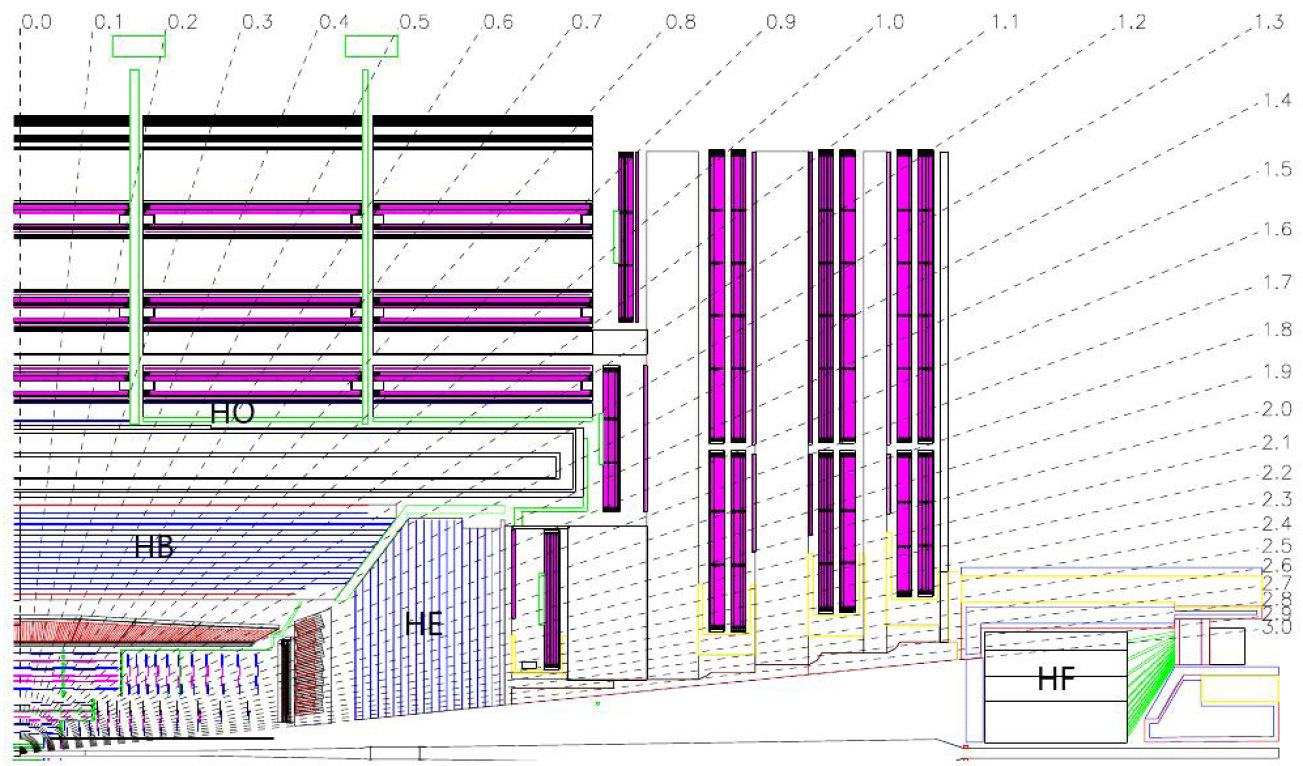
\includegraphics[width=0.65\textwidth]{figures/experiment/CMS/fig_HCALdiagram_smaller_size.png}
  \caption{A quarter section of the CMS detector including the HCAL in a transverse view. Taken from~\cite{bib:CMS:experiment}.}  
  \label{fig:HCAL}
\end{figure}

The HCAL is dedicated to measuring the energy of hadrons as well as improving the estimate of the missing energy in the event because of its large pseudorapidity coverage.
The latter one is achieved by the high pseudorapidity coverage ($|\eta|<5.0$) that assures the detection of most of the visible particles.

The HCAL is a so-called sampling calorimeter which consists of brass absorber material, initiating the hadronic shower, as well as active plastic scintillators.
The emitted photons are read out with wavelength-shifting (WLS) fibres which are embedded into the scintillators.
These in turn are connected to fibres that transfer the light to the readout system.

The hadron barrel (HB) covers the pseudorapidity range between $-1.4 < \eta < 1.4$.
It is composed of 17 layers of absorber material (15 brass and 2 steel layers) interleaved with scintillator layers.
The scintillator layers are divided into 2304 towers with a size of $\Delta \eta \times \Delta \phi = 0.087 \times 0.087$.

The hadron outer (HO) covers a pseudorapidity range up to $|\eta|=1.26$.
It is located between the solenoid and the barrel detector of the muon system.
The HO is dedicated to measuring the energy of the shower leakage of hadrons.
Its thickness corresponds to over ten interaction lengths.

The hadron endcap (HE) extends the pseudorapidity coverage of the HCAL up to $|\eta|=3.0$ and starts at $|\eta|=1.3$.
It consists of 2304 towers in total, which vary in size between $5-10\degree$ in the $\phi$ direction and $0.087-0.35$ in $\eta$ direction.

Finally, the hadron forward (HF) calorimeter extends the pseudorapidity range up to $|\eta|=5.0$, starting from $|\eta|=3.0$.
It is build out of steel plates with $1\mm^2$ grooves containing quartz fibres.
The emitted light by the quartz fibres is transferred to photomultipliers.
The HF is divided into 13 towers where almost all towers have a spread of $\Delta \eta \approx 0.175$ in $\eta$ direction and $\sim 10\degree$ in $\phi$ direction.
 
%%%%%%%%%%%%%%%%%%%%%%%%%%%%%%%%%%%%%%%%%%%%%%%%%%%%%%%%%%%%%%%%%%%%%%%%%%%%%%%%%%%%%%%%%%%%%%%%%%%%%%%%%%%%%%%%%%%%%%%%%%%%%%%%%%%%%%%%%%%%%%%%%%%%%%%%%%%%%%%%%%%%%%%%%%%%%%%%%%%%%%%%%%%%%%%%%%%%%%%%%%%%%%%%%%%%%%%%%%%%%%%%%%
\section{The muon system}
\label{sec:MuonSystem}
The muon system~\cite{bib:CMS:TDR_2006,bib:CMS:TDR_MuonSystem} is the outermost component of the CMS detector.
It comprises three different types of gaseous detectors, mounted into the iron return yokes: drift tube (DT) chambers in the barrel region ($|\eta|<1.2$), cathode strip chambers (CSC) in the endcap region ($1.04<|\eta|<2.4$) and resistive plate chambers (RPC) in the barrel as well as the endcap region ($|\eta|<1.6$) (see Fig.~\ref{fig:MuonSystem} for a schematic sketch of the muon system).
\begin{figure}[!b]
  \centering
      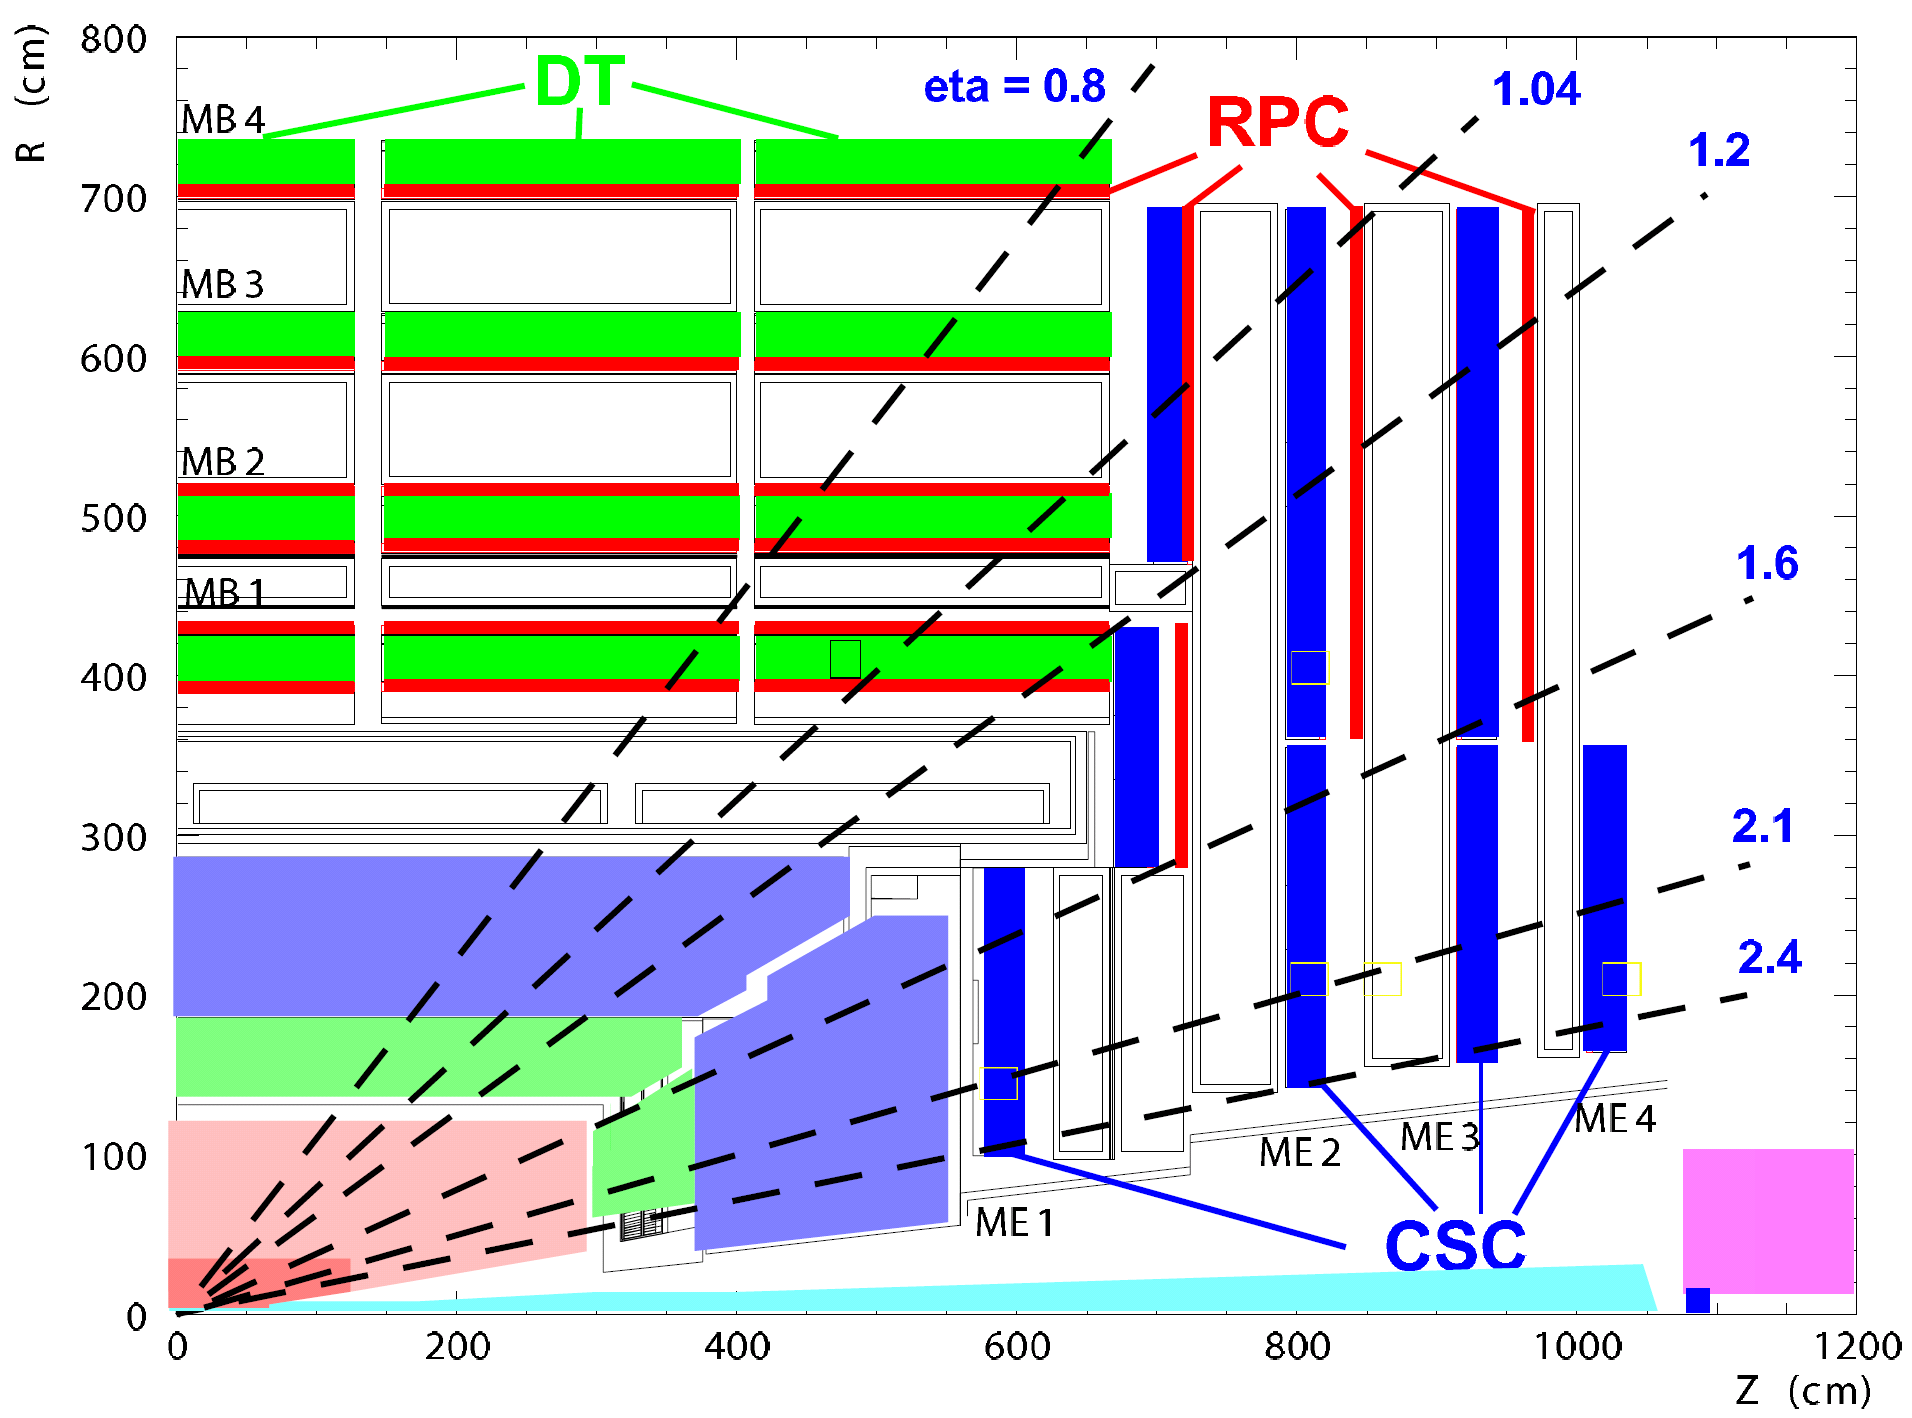
\includegraphics[width=0.60\textwidth]{figures/experiment/CMS/Figures_Experimental_Apparatus_MuonDetector.png}
  \caption{A quarter section of the CMS detector in the transverse plane with a detailed view on the muon system. Taken from~\cite{bib:CMS:TDR_2006}.}  
  \label{fig:MuonSystem}
\end{figure}
In the barrel part of the muon system, four layers (so-called stations) of drift-tube chambers are assembled inside the iron return yoke layers at radii of 4.0, 4.9, 5.9 and 7.0\m from the beam axis.
The position of a muon traversing these layers can be measured with a precision of $\approx 100\mum$ in radial direction and $\approx 1\,$mrad in $\phi$ direction. 

The four endcap disks are made up of 468 cathode strip chambers in total.
By measuring the centre-of-gravity, they achieve a spatial resolution of $\approx 100-200\mum$ and an angular resolution of $\approx 10\,$mrad in $\phi$ direction.
They are designed in order to cope with a high particle flux of about 1kHz/cm$^2$ and a non-uniform magnetic field.
As signals can be transferred very fast, they are used for the level-1 trigger system (see Section~\ref{sec:TriggerSystem}).

Finally, the resistive plate chambers cover the barrel as well as the endcap region up to a pseudorapidity of $\eta=1.6$. 
They provide a fast response with a good time resolution enabling the exact identification of the respective bunch-crossing.
It is used for the level-1 trigger system as well.
%%%%%%%%%%%%%%%%%%%%%%%%%%%%%%%%%%%%%%%%%%%%%%%%%%%%%%%%%%%%%%%%%%%%%%%%%%%%%%%%%%%%%%%%%%%%%%%%%%%%%%%%%%%%%%%%%%%%%%%%%%%%%%%%%%%%%%%%%%%%%%%%%%%%%%%%%%%%%%%%%%%%%%%%%%%%%%%%%%%%%%%%%%%%%%%%%%%%%%%%%%%%%%%%%%%%%%%%%%%%%%%%%%
\section{The trigger system}
\label{sec:TriggerSystem}
Because of the impossibility of storing each event occurring at the CMS experiment (cf. bunch crossing rate of 20\mhz), a multistage trigger system~\cite{bib:CMS:TDR_2006} is used to achieve a drastic reduction of recorded events by nearly six orders of magnitude.
It comprises two main parts: a so-called level-1 (L1) trigger system and a high-level trigger (HLT) system.

The L1 triggers need to provide a very fast decision (3.2\mus, where around 1\mus is allocated to the actual L1 trigger calculations) whether an event shall be recorded or not.
During this time, the recorded event data is held in buffers located close to the single detector components.
Information from the muon system and the calorimeters is used for the L1-trigger decisions.
Objects used for these decisions are so-called ``trigger primitive'' objects: photons, electrons, muons, jets above certain \et and \pt thresholds and global variables like missing transverse energy, \met. 
The design value of the number of events per second that pass this trigger stage is 100\khz.

After a time of 3.2\mus, the stored data in the buffers close to the single detector components are transferred to the front-end readout buffers in case the event passed the L1-trigger requirements.
By partial event reconstruction and the use of various detector signals (calorimeter, muon information followed by pixel information and full event reconstruction), higher event objects can be used to check whether HLT-trigger requirements are fulfilled.
On HLT level, the decision time amounts to 50\ms and a reduction from 100\khz to 100\hz of event recording is achieved.

%%%%%%%%%%%%%%%%%%%%%%%%%%%%%%%%%%%%%%%%%%%%%%%%%%%%%%%%%%%%%%%%%%%%%%%%%%%%%%%%%%%%%%%%%%%%%%%%%%%%%%%%%%%%%%%%%%%%%%%%%%%%%%%%%%%%%%%%%%%%%%%%%%%%%%%%%%%%%%%%%%%%%%%%%%%%%%%%%%%%%%%%%%%%%%%%%%%%%%%%%%%%%%%%%%%%%%%%%%%%%%%%%%%
%%%%%%%%%%%%%%%%%%%%%%%%%%%%%%%%%%%%%%%%%%%%%%%%%%%%%%%%%%%%%%%%%%%%%%%%%%%%%%%%%%%%%%%%%%%%%%%%%%%%%%%%%%%%%%%%%%%%%%%%%%%%%%%%%%%%%%%%%%%%%%%%%%%%%%%%%%%%%%%%%%%%%%%%%%%%%%%%%%%%%%%%%%%%%%%%%%%%%%%%%%%%%%%%%%%%%%%%%%%%%%%%%%%
%%%%%%%%%%%%%%%%%%%%%%%%%%%%%%%%%%%%%%%%%%%%%%%%%%%%%%%%%%%%%%%%%%%%%%%%%%%%%%%%%%%%%%%%%%%%%%%%%%%%%%%%%%%%%%%%%%%%%%%%%%%%%%%%%%%%%%%%%%%%%%%%%%%%%%%%%%%%%%%%%%%%%%%%%%%%%%%%%%%%%%%%%%%%%%%%%%%%%%%%%%%%%%%%%%%%%%%%%%%%%%%%%%%
\FloatBarrier
\chapter{Event reconstruction and particle identification}
A crucial ingredient of data analysis at the CMS experiment is the translation of the signal measurements in the various sub-detector components into physical objects, like muons, electrons, etc..
For this translation, \ie for particle identification, information from all detector components is used.
This is known as the particle-flow event reconstruction algorithm~\cite{CMS-PAS-PFT-09-001}.
In Fig.~\ref{fig:CMSslice}, a slice through the CMS detector is shown with the signatures of different particles indicated as coloured lines.

In the next section an introduction to this algorithm is given, followed by the definition and classification of physics objects at the CMS experiment.
\begin{figure}[!ht]
  \centering
      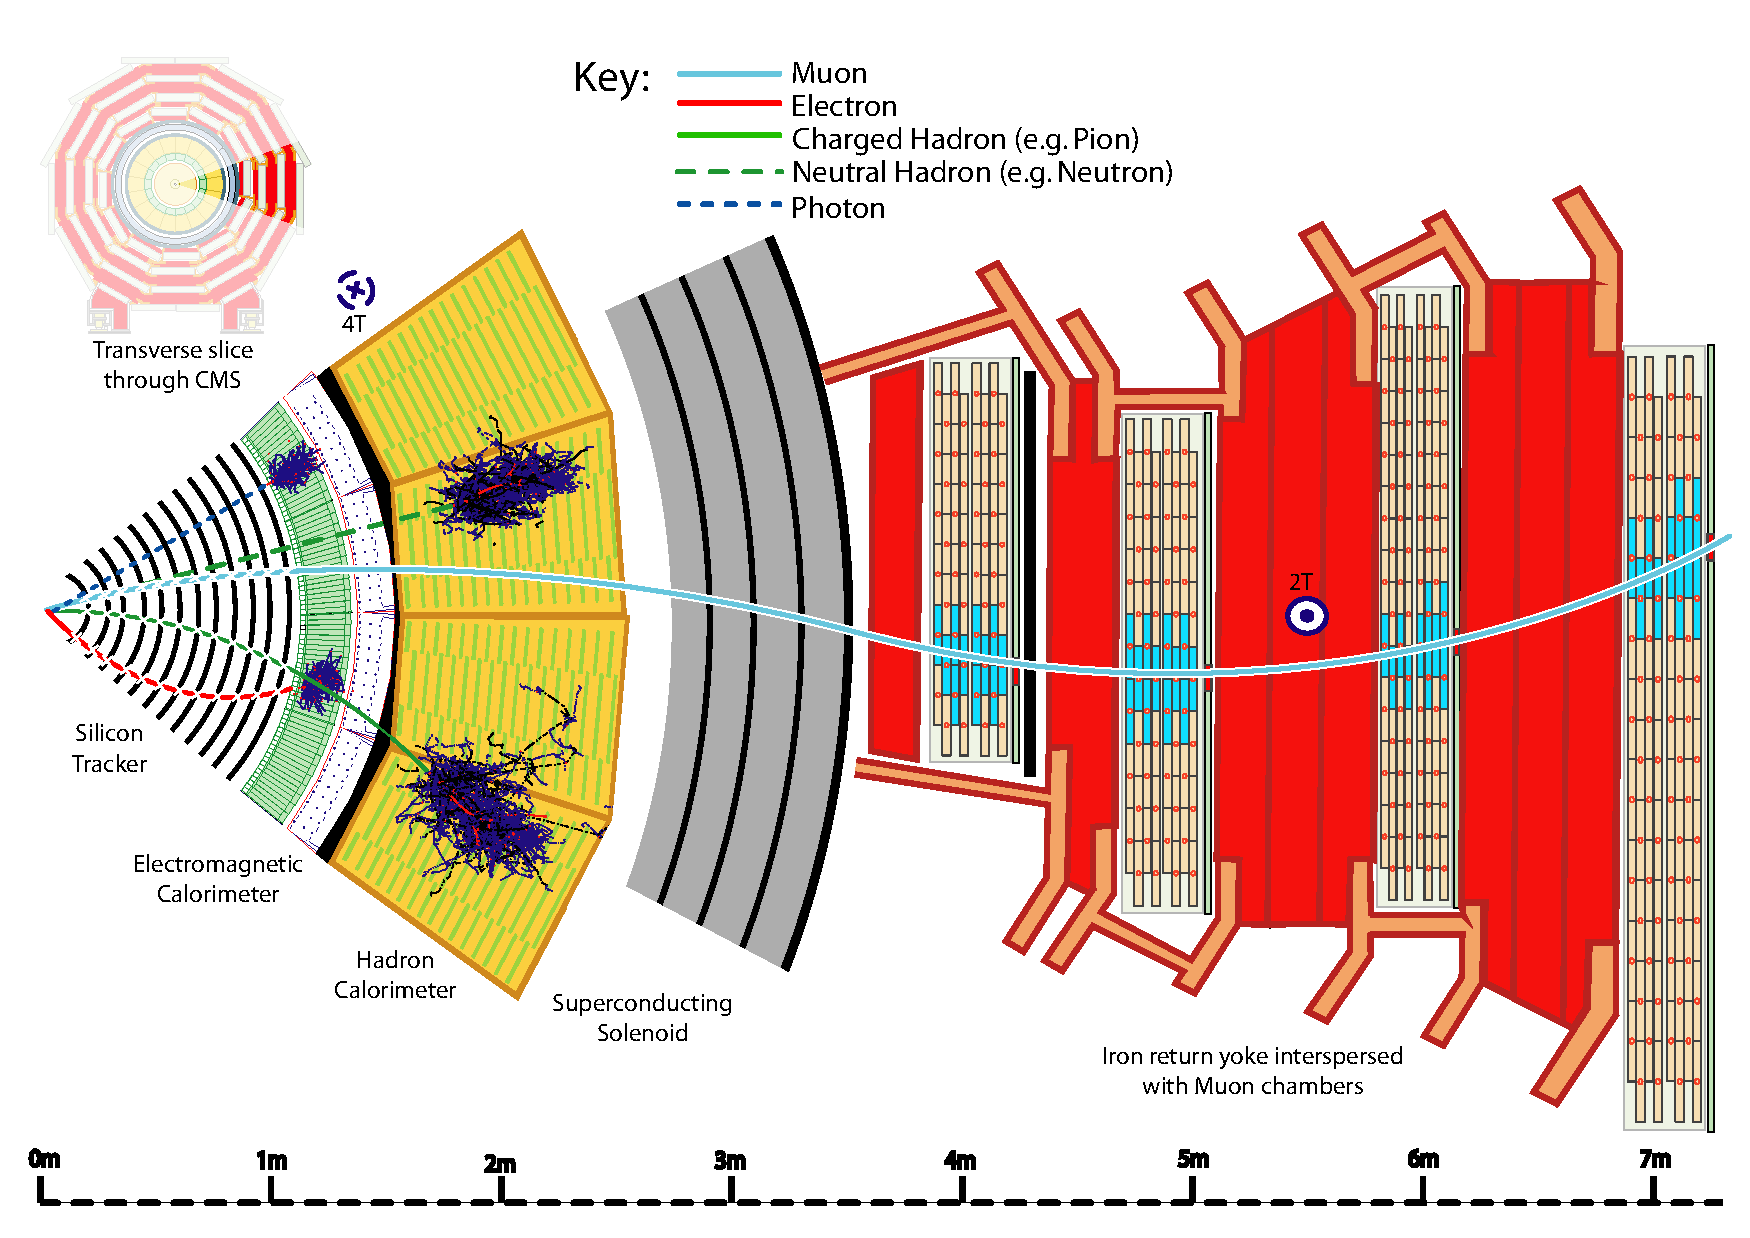
\includegraphics[width=0.99\textwidth]{figures/experiment/ObjectReconstruction/slice_white_smaller_size.pdf}
  \caption{A radial slice through the CMS detector with several particle signatures indicated as coloured lines. Taken from~\cite{bib:Signatures_figure}.}  
  \label{fig:CMSslice}
\end{figure}


\section{The particle-flow algorithm}
\label{sec:PFalgorithm}
The particle-flow (PF) event description~\cite{CMS-PAS-PFT-09-001} aims at optimising particle identification and reconstruction by the usage of all sub-detector components of the CMS detector.
There are three main building bricks used for global event description: reconstructed charged-particle tracks, calorimeter clusters, and muon tracks.
The main requirements for these building bricks are a high reconstruction efficiency and a small fake rate.
Therefore, a special emphasis was put on developing a very efficient tracking algorithm (see Section~\ref{sec:ObjectReconstruction}) and a well performing calorimeter clustering algorithm~\cite{CMS-PAS-PFT-09-001}. 

The particle-flow algorithm proceeds as follows for each event (the description is based on~\cite{CMS-PAS-PFT-09-001}):
\begin{enumerate}
\item For each pair of detected building bricks, a ``link distance'' is calculated in order to quantify the quality of their link, \ie whether the two building bricks stem from the same particle. 
\item ``Blocks'' are produced from the building bricks that are linked together (with a typical number of one, two or three building bricks contained in a block) using different algorithms for different sets of building bricks (see~\cite{CMS-PAS-PFT-09-001} for detailed information about these algorithms).
      Blocks comprise either charged-particle tracks and calorimeter clusters, or several calorimeter clusters, or a charged-particle track in the tracker and a muon track in the muon system.
      The latter is called a global muon.
\item For each block the following steps are performed:
\begin{enumerate}
\item Each global muon where the \pt measured in both sub-detectors is compatible with the  \pt  measurement in the tracker is defined as a particle-flow muon and the track in both sub-detectors is removed from the block.
\item Next, electrons are reconstructed and identified using tracker hits and ECAL clusters. 
      For an identified particle-flow electron, the corresponding tracker hits and the ECAL clusters (including energy deposits from Bremsstrahlung photons) are removed from the block. 
\item Tighter track quality criteria are applied.
\item The compatibility of the remaining ECAL and HCAL energy deposits to the transverse momentum of the reconstructed tracks within a block is checked. 
      This allows for the identification of particle-flow charged hadrons with a momentum estimate using tracker and calorimeter information. 
      If the energy deposits in the ECAL or HCAL are much larger than the corresponding track \pt, the signature is identified as a particle-flow photon or particle-flow neutral hadron, respectively. 
      All ECAL and HCAL clusters used for the identification as well as the reconstructed tracks are removed from the block.
\item Finally, the remaining ECAL and HCAL clusters (which are all not linked to any other building block) are identified as particle-flow photons or particle-flow neutral hadrons, respectively.
\end{enumerate}
\end{enumerate}
For the final identification of particles and other objects further reconstruction criteria are applied (see Section~\ref{sec:ObjectReconstruction}).

\section{Object reconstruction}
\label{sec:ObjectReconstruction}
In this section, an overview of the required criteria for the identification of particles and other physics objects is given.

\subsection{Reconstruction of primary vertices} 
\label{sec:VertexReconstruction}
The reconstruction of primary vertices (PVs) is important in order to determine the location of the interaction point and to get an estimate of the corresponding uncertainty.
At the CMS experiment, the reconstruction of vertices proceeds as follows~\cite{bib:CMS:tracking_8TeV}:
First, a track selection is performed which depends on the number of hits in the tracker, on the significance of the transverse distance to the beam spot ($|d_0^{\text{BS}}|/\delta d_0$), and the normalised $\chi^2$ of the track fit (see the subsequent Section~\ref{subsec:TrackReconstruction} for more information on the track reconstruction algorithms).
All selected tracks are afterwards clustered to several vertices based on their point of closest approach in $z$-direction to the beam spot.
The clustering first identifies candidate vertices using a so-called deterministic annealing (DA) algorithm~\cite{bib:VertexReconstruction_DA}.
Subsequently, the candidate vertices are evaluated with the adaptive vertex fitter~\cite{bib:VertexReconstruction_AVF}, which estimates the location of the vertices as well as performance parameters of the fit.
A weight is assigned to each track that is close to one in case for a good compatibility and close to zero for a bad compatibility with the vertex.
The track with the largest sum of all squared track transverse momenta, $\sum \pt^2$, is referred to as the primary vertex. 
All other vertices during a bunch-crossing are so-called pileup interactions.

Further quality criteria of the primary vertex are required in the search for highly ionising, short tracks (Part~\ref{part:analysis}) and the measurement of the jet transverse-momentum resolution (Part~\ref{part:resolution}).
For this purpose, the ``number of degrees of freedom'' of the primary vertex is introduced: 
\begin{equation}
n_{\text{dof}} = -3 + 2 \sum_{\text{tracks}} w_i.
\end{equation}
The requirement of a well reconstructed primary vertex is  $n_{\text{dof}}>4$.
Furthermore, the vertex is required to be within 24\cm in $z$- and 2\cm in $r$-direction with respect to the nominal interaction point.


\subsection{Reconstruction of tracks}
\label{subsec:TrackReconstruction}
The reconstruction of tracks aims at linking several hits in the tracking system to one reconstructed track that matches the original trajectory of the particle with a high probability.
With the track reconstruction, an estimate of the particle momentum as well as its position can be achieved.
Track reconstruction is challenging because the large number of hits\footnote{At design luminosity around 1000 charged particles are expected to traverse the tracker in each bunch-crossing~\cite{bib:CMS:tracking_8TeV}}, especially in the layers close to the interaction vertex, leads to a high combinatorial complexity. 
In the following, an overview of the tracking algorithm used at CMS is given.
It is based on~\cite{bib:CMS:tracking_8TeV} and the reader is referred to this reference for more information on the reconstruction of tracks at CMS.\\

The tracking software used at CMS is usually referred to as the Combinatorial Track Finder (CTF).
It it based on the so-called combinatorial Kalman filter~\cite{bib:TrackAlgorithm_1989,bib:TrackAlgorithm_1990,bib:TrackAlgorithm_1997} which in turn is based on the Kalman filter~\cite{bib:KalmanFilter_1987}.
The Kalman filter is an algorithm that allows for the estimation of parameters of interest based on a set of observations that are subject to noise or other inaccuracies.
It is mathematically equivalent to a global least square minimisation for linear models with Gaussian noise.

The basic idea of the tracking algorithm at CMS is to avoid applying the combinatorial Kalman filter on all hits in one step by using an iterative procedure (called iterative tracking).
A reduction of complexity can be achieved by first reconstructing tracks that are easy to identify because of \eg a relatively high \pt. 
These tracks are removed afterwards and the remaining tracker hits are subject to further reconstruction iterations.
The following iterations are performed (these steps refer to the setting from May to August in 2011 but are in their basic structure retained in the year 2012):
\begin{itemize}
\item Iteration 0: Tracks near the \pp-interaction point that have three pixel hits and a $\pt>0.8\gev$ are reconstructed.
\item Iteration 1: Tracks with only two pixel hits and $\pt>0.8\gev$ are reconstructed. 
\item Iteration 2: Low \pt tracks from the \pp-interaction point are reconstructed.
\item Iteration 3-5: Reconstruction of tracks that are not originating from the primary vertex or that were not found by previous iterations.
\end{itemize}
Within these iterations, the reconstruction is subdivided into four different steps:
\begin{itemize}
\item Seed generation: Only 2-3 hits are used to define track candidates.
\item Extrapolation: Based on the expected flight path, additional hits are assigned to the candidate track using a combinatorial Kalman filter.
\item Track fitting: With the usage of the Kalman filter and a smoother, the trajectory is fitted in order to estimate the track parameters.
\item Setting of quality flags: Quality flags are assigned to all tracks and tracks that fail certain quality criteria are discarded.\\
\end{itemize}
%The configuration of the first and the fourth step differs across the different iterations.  

A special task when reconstruction tracks consists of the suppression of fake tracks, \ie tracks that are not associated with a charged particle.
Therefore, the requirement of fulfilling certain quality criteria (fourth step) is crucial to substantially reduce the contamination of fake tracks.
 For this purpose, requirements on the following variables are imposed (the values of the parameters $\alpha$ and $\beta$ vary across iterations):
\begin{itemize}
\item A minimum number of layers in which the track has an associated hit.
\item A minimum number of layers in which the track has an associated 3D hit\footnote{A 3D hit refers to a measurement that provides 3D position information, such as a pixel hit or a strip hit in a stereo module.}.
\item A maximum number of layers in which the track has no associated hit.
\item A high quality of the trajectory fit: $\chi^2/\text{ndof} < \alpha_0 N_{\text{layers}}$.
\item A low transverse impact parameter significance:  $|d_0^{\text{BS}}|/\delta d_0 < \left( \alpha_3 N_{\text{layers}} \right)^{\beta}$,\\
\hspace*{231pt}                                        $|d_0^{\text{BS}}|/\sigma_{d_0} \left(\pt\right) < \left( \alpha_1 N_{\text{layers}} \right)^{\beta}$.
\item A low longitudinal impact parameter significance: $|z_0^{\text{PV}}|/\delta z_0 < \left( \alpha_4 N_{\text{layers}} \right)^{\beta}$\\
\hspace*{240pt}                                         $|z_0^{\text{PV}}|/\sigma_{z_0} \left(\pt,\eta\right) < \left( \alpha_2 N_{\text{layers}} \right)^{\beta}$.
\end{itemize}
The variable $d_0^{\text{BS}}$ is the distance of the track to the centre of the beam spot in the transverse plane to the beam line and $z_0^{\text{PV}}$ is the distance along the beam line to the closest pixel.
The variables $\delta d_0$ and $\delta z_0$ are the uncertainties on the distance (impact) parameters and $\sigma$ is the standard deviation corresponding to the length of the beam spot in z-direction.



\subsection{Reconstruction of jets} 
\label{sec:JetReconstruction}
In Section~\ref{sec:PFalgorithm}, the reconstruction of particle-flow neutral and charged hadrons was already introduced.
Charged and neutral hadrons are usually formed in the hadronisation process of final state quarks and gluons.
Since the interest at particle colliders concerns the sum of all particles arising from one final state gluon or quark, which is referred to as a jet, the reconstruction of jets is a very important task at particle colliders.
Foremost, the clustering of the particle-flow candidates to a jet is a crucial ingredient for the reconstruction of jets.
Furthermore, the calibration of the measured jet transverse momentum as well as the subtraction of energy due to pileup interactions is important to ensure a good quality \pt measurement of jets at CMS.
All three subjects are explained in detail in the following sections.
\subsubsection*{Clustering of jets}
%As already noted, jets are formed by quarks or gluons in the final state that hadronise due to colour confinement. 
%The reconstruction of jets is therefore subject to a clustering algorithm that clusters reconstructed particle-flow objects into a jet.
%At CMS, the so-called \antikt cluster algorithm~\cite{bib:JetClustering_2008} is used.
The clustering algorithm used at the CMS experiment belongs to the class of sequential recombination jet algorithms.
In sequential recombination algorithms, a distance measure between two particles - or more generally objects - is used to cluster them into jet cones.
For this purposes, two quantities are defined
\begin{equation}
\begin{aligned}
\label{eq:Antikt}
d_{ij} &= \text{min}\left( p_{\text{T,}i}^{2k},p_{\text{T,}j}^{2k} \right) \frac{\Delta_{ij}^2}{R^2},\\
d_{iB} &= p_{\text{T,}i}^{2k},
\end{aligned} 
\end{equation}
with $\Delta_{ij}$ referring to the distance between particles $i$ and $j$ in the $\eta - \phi$ plane and $R$ denoting the radius parameter of the algorithm which determines the cluster scale.
The quantity $k$ can be any integer and specifies the behaviour of the algorithm, as will be seen later.
The algorithm is an iterative procedure comprising the following steps: 
First, the quantities $d_{iB}$ and $d_{ij}$ are calculated for every single and every pair of ``objects'' in the event, respectively.
An object can be a particle or a set of already clustered particles.
If the smallest quantity is a distance between a pair of objects, these objects are clustered together.
If the smallest quantity is $d_{iB}$, the corresponding object is considered a jet and removed from the object list.
If all objects are removed from the input list of the algorithm, the clustering comes to an end.

As noted before, the integer $k$ in Eq.~\eqref{eq:Antikt} defines different types of algorithms.
For the choice of $k=0$, the algorithm is referred to as Cambridge/Aachen algorithm~\cite{bib:Cambridge_1997,bib:Cambridge_1998}.
It doesn't take the momentum of particles into account for the clustering but is only based on spatial information.
The \kt algorithm~\cite{bib:kT_algorithm_1993,bib:kT_algorithm_Ellis} uses the configuration with $k=1$, thus starting the clustering with low momentum particles.
At CMS, the \antikt algorithm is used with $k=-1$. 
It begins with clustering high momentum particles and leads to very regular shapes of the jet cones.
The behaviour of the three different clustering algorithm is illustrated in Fig.~\ref{fig:ClusteringAlgorithms}. 
One single parton-level event was subject to the three different jet clustering algorithms.
Roughly 1000 soft particles are added to the event in order to test the adaptiveness of the jet algorithms to soft particles.
It can be seen, that the Cambridge/Aachen and the \kt algorithm are both more irregular in shape, while jets clustered with the \antikt method result in circular shapes.
\begin{figure}[!t]
  \centering
      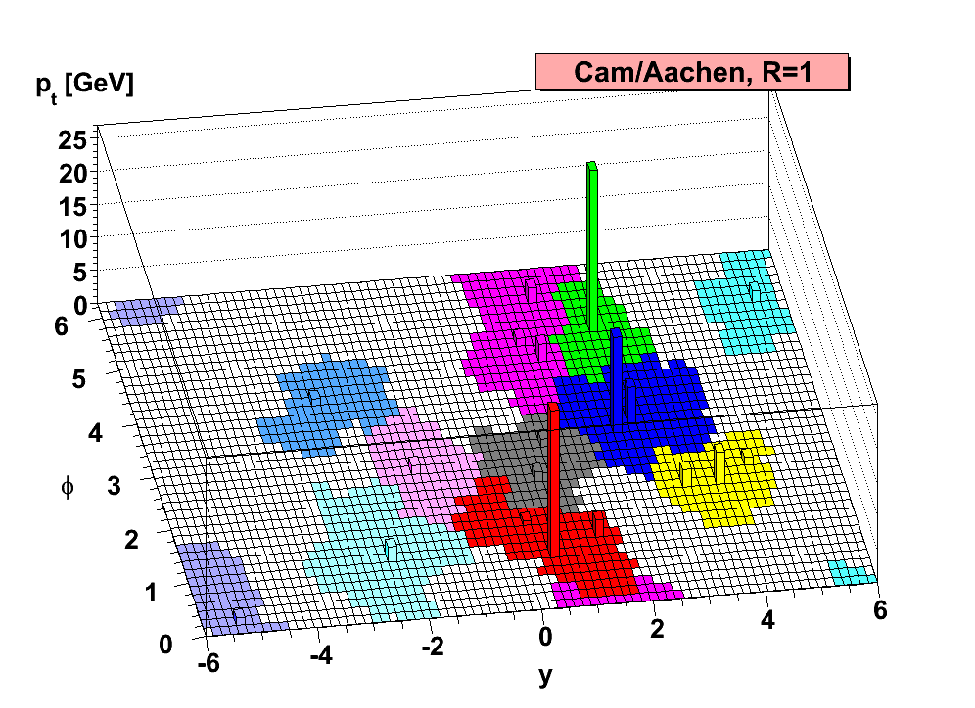
\includegraphics[width=0.32\textwidth]{figures/experiment/ObjectReconstruction/herwig-parton-level-ev-cam.pdf}
      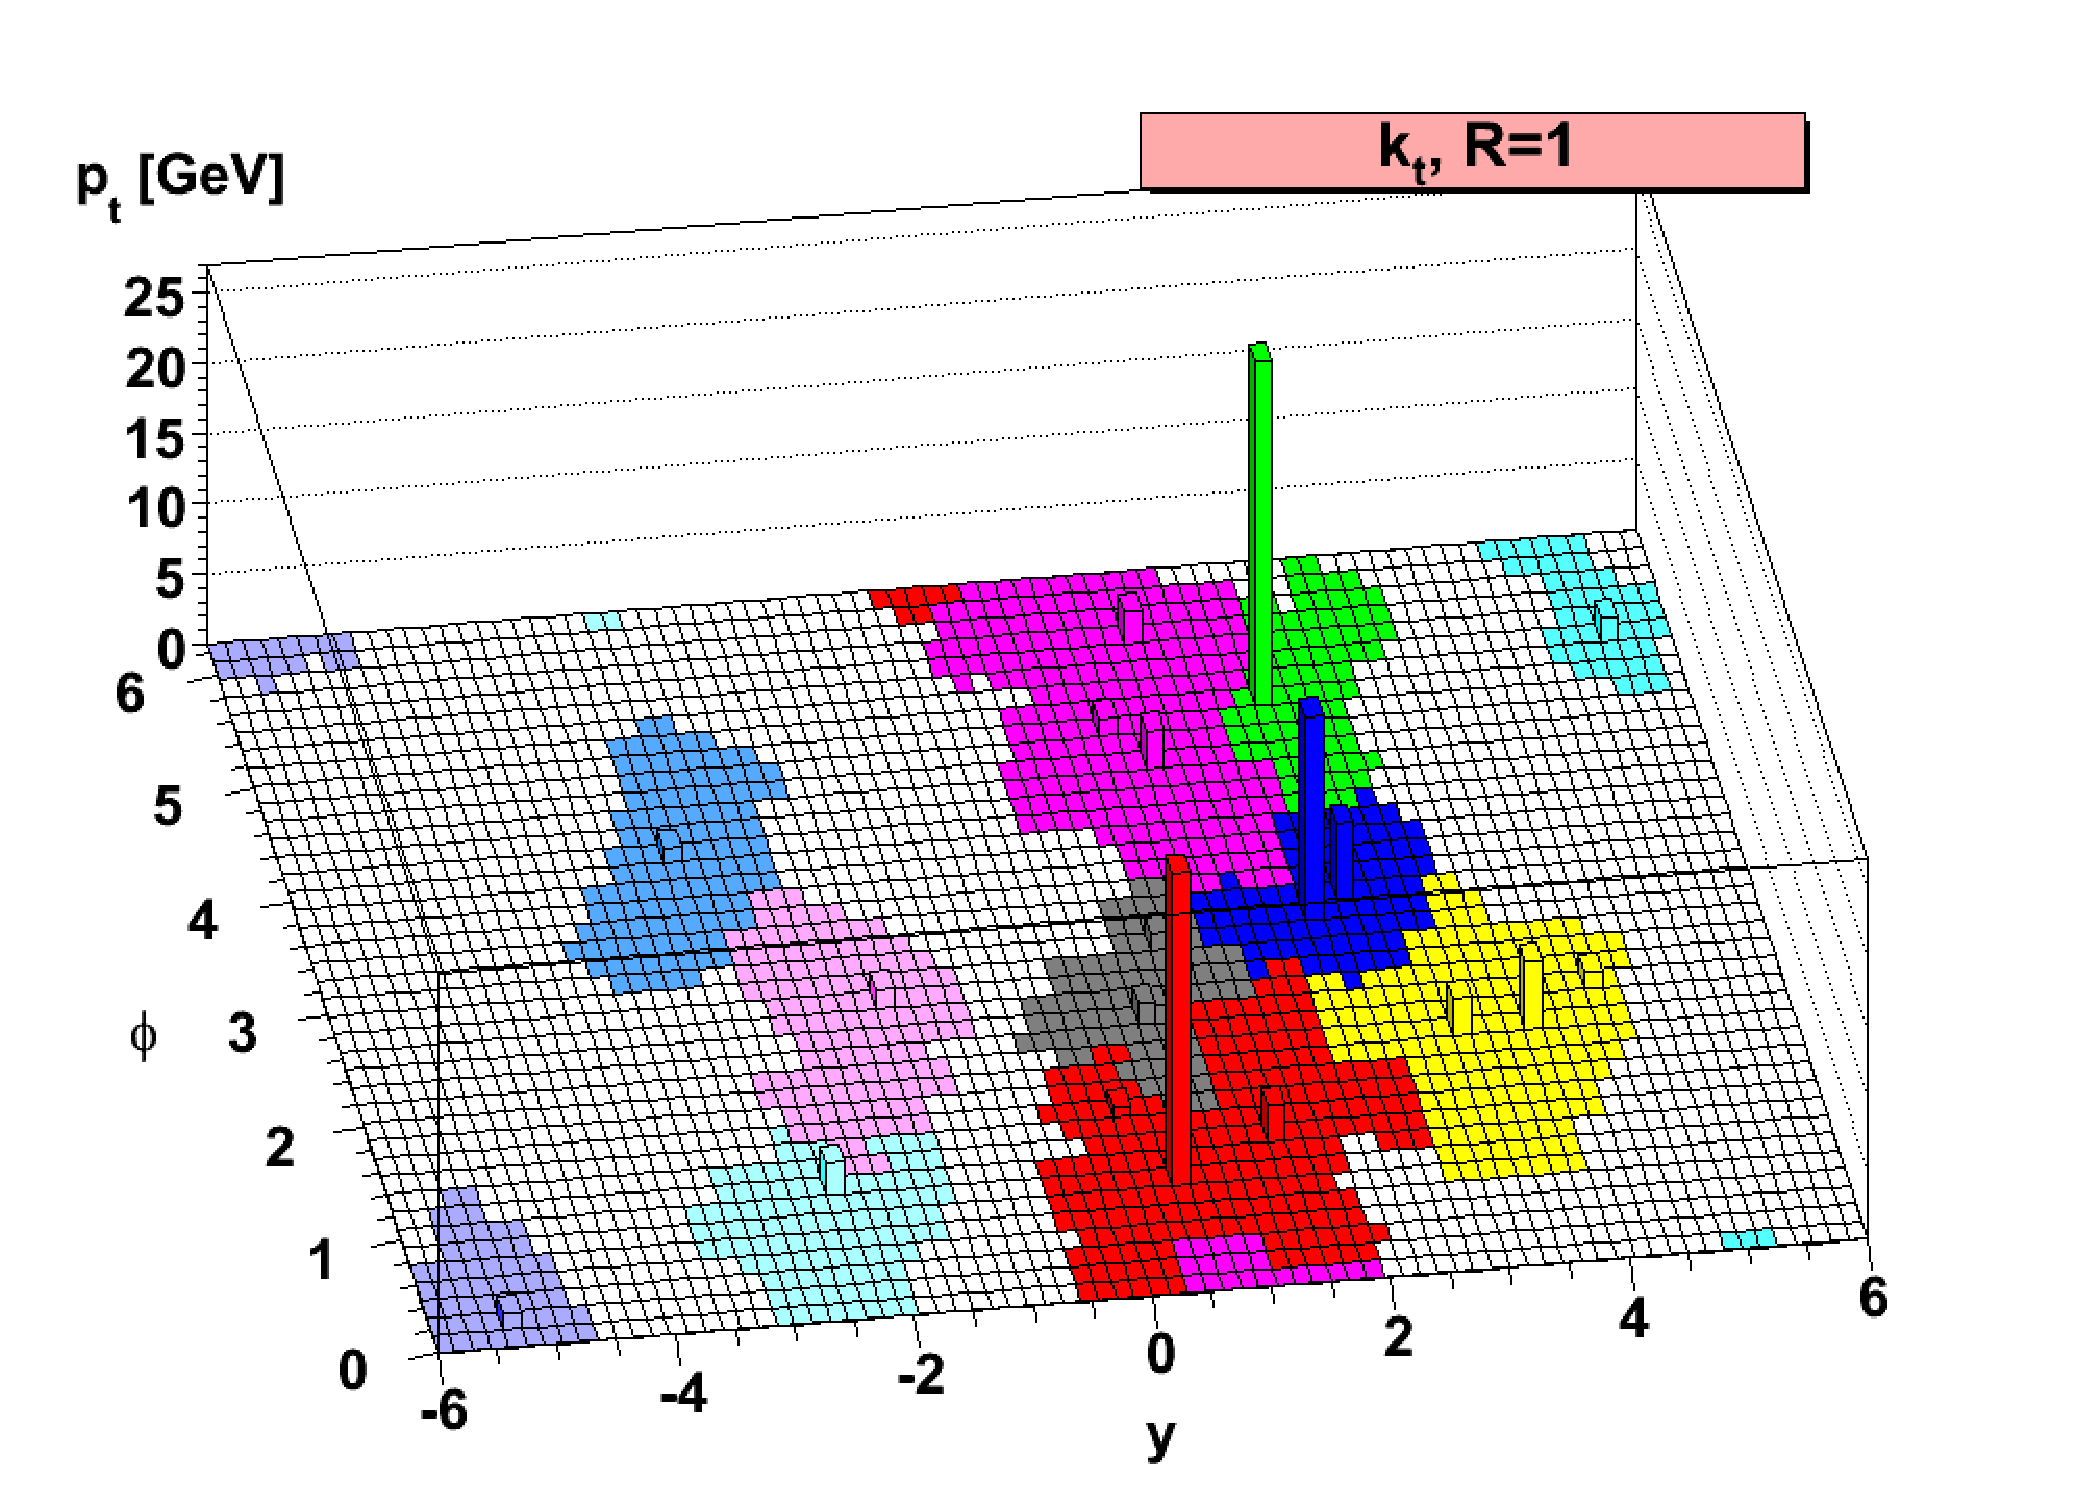
\includegraphics[width=0.32\textwidth]{figures/experiment/ObjectReconstruction/herwig-parton-level-ev-kt.pdf}
      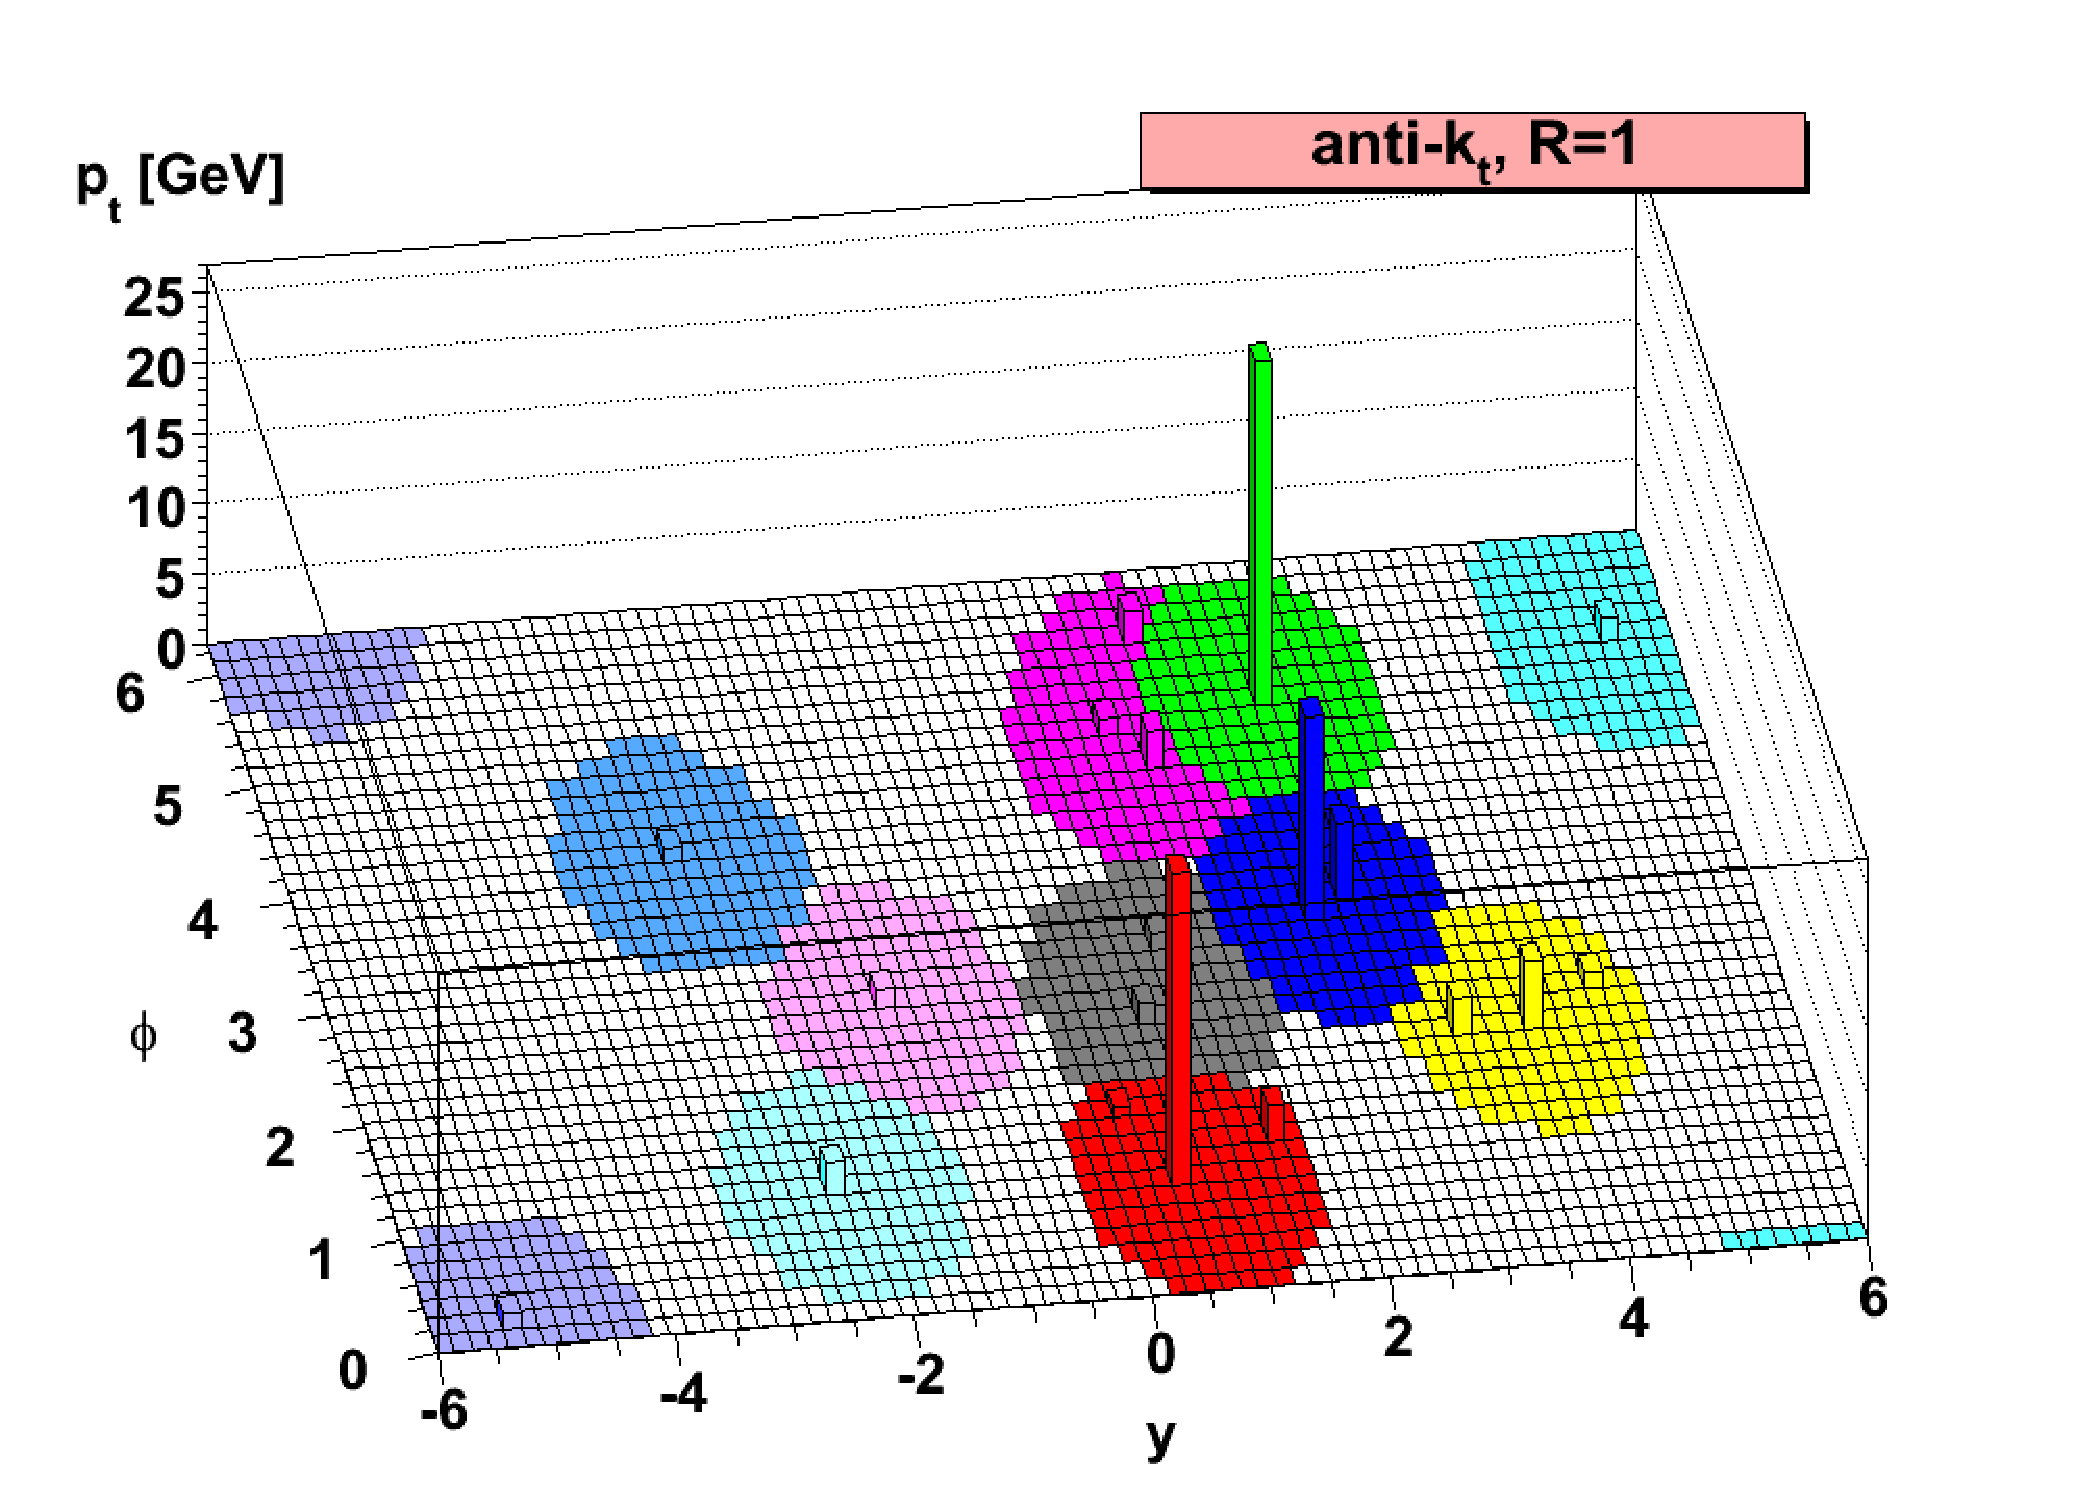
\includegraphics[width=0.32\textwidth]{figures/experiment/ObjectReconstruction/herwig-parton-level-ev-antikt.pdf}
  \caption{Parton-level event in the $\eta - \phi$ plane with $\sim 1000$ soft particles added. Three different algorithms are used to cluster the particles into jet cones (coloured areas): the Cambridge/Aachen algorithm (left), the \kt algorithm (middle), and the \antikt algorithm (right). Taken from~\cite{bib:JetClustering_2008}.}  
  \label{fig:ClusteringAlgorithms}
\end{figure}
Furthermore, jets clustered with sequential recombination jet algorithms are infrared and collinear safe.

Throughout this thesis jets clustered with the \antikt algorithm with a radius parameter of $R=0.5$ are used.

\subsubsection*{Jet energy calibration}
In order to account for possible mismeasurements of the jet transverse momentum, all jets at CMS are subject to a calibration procedure.
This calibration aims at eliminating discrepancies between the measured jet \pt and the true jet \pt because of pileup interactions (level-1 corrections) as well as discrepancies depending on jet \pt and $\eta$ (level-2 and level-3 corrections). 
The calibration factors of the level-1, level-2 and level-3 corrections are determined fully in simulation.
To ensure also a complete calibration of jets in data, additional correction factors are determined which are only applied on the jet \pt measured in data (level-2 and \mbox{level-3} residual corrections).
These calibration factors are determined with the help of reference objects in data, such as photons.
An overview of the applied correction factors in simulation and data is shown in Fig.~\ref{fig:JetEnergyCorrections}.
\begin{figure}[!b] 
  \centering
      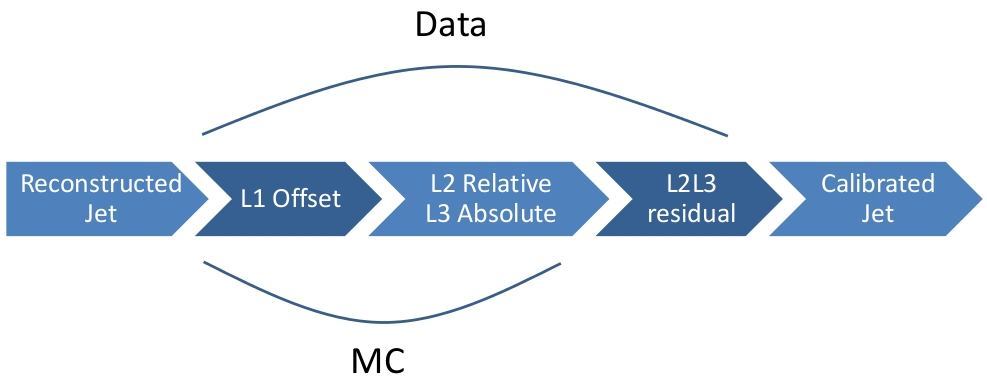
\includegraphics[width=0.99\textwidth]{figures/experiment/ObjectReconstruction/JEC.jpg}
  \caption{Visualisation of the various steps of the jet energy calibration at the CMS experiment. The lines embrace the applied calibration steps for simulation (MC) and data. Taken from~\cite{bib:Kristin_Thesis}.}  
  \label{fig:JetEnergyCorrections}
\end{figure}

In the following, a more detailed description of the determination of the factorised calibration factors will be given.
For an extensive description of the calibration approach, the reader is referred to~\cite{bib:CMS:JERCPaper_2011}
\begin{description}
\item \textbf{L1 pileup offset corrections:} In order to eliminate a mismeasurement of the jet \pt because of pileup interactions, correction factors ($C_{\mathrm{offset}}$) are determined that are supposed to restore the true jet \pt. This correction is determined in bins of jet \pt, jet $\eta$, the jet area $A$, and the event energy density $\rho$. The correction factors are determined with simulated samples and are applied to measured data as well as simulated events.
\item \textbf{L2 relative + L3 absolute corrections:} These two corrections are devoted to correct the measured jet \pt in order to ensure a uniform response ($\ptrecojet/\pttruejet$) vs. \mbox{$\eta$ (L2)} ($C_{\mathrm{rel}}$) and \mbox{\pt (L3)} ($C_{\mathrm{abs}}$). They are also determined in simulated samples and applied to simulated and measured events.
\item \textbf{L2L3 residual corrections:} Finally, correction factors ($C_\mathrm{res}$) are determined in order to remove any residual bias in data. They are estimated in data with the help of QCD-multijet events to ensure a uniform response vs. $\eta$ (L2) and with $\gamma/Z+$ jets events in order to ensure a uniform response vs. \pt (L3).
These factors are not applied to simulation.\\
\end{description}

The derived correction factors are applied on the measured transverse momentum in a factorised approach according to the following equation:
\begin{equation}
\pt^\mathrm{cor} =  C_\mathrm{res}(\pt'', \eta) \cdot C_{\mathrm{rel}}(\eta) \cdot C_{\mathrm{abs}}(\pt') \cdot C_{\mathrm{offset}}(\pt^\mathrm{raw}, \eta) \cdot  \pt^\mathrm{raw},
\end{equation}
where $\pt^\mathrm{cor}$ is the corrected jet \pt and  $\pt^\mathrm{raw}$ is the fully uncorrected jet \pt.
By the application of the various correction factors, the jet transverse momentum is calibrated in a factorised manner.

Throughout this thesis, all jets are calibrated by the application of the jet transverse momentum correction factors, referred to as jet energy corrections.


\subsubsection*{Charged hadron subtraction}
Particles originating from pileup vertices (additional vertices during a bunch crossing) can be clustered into jets leading to higher energies of the reconstructed jet.
Therefore a procedure called charged hadron subtraction (CHS) is applied.
It removes reconstructed charged particles that do not originate from the primary vertex (see~\cite{bib:CHS_2012} for more details).

In this thesis, all jets are subject to charged hadron subtraction.

\subsection{Reconstruction of photons}
\label{subsec:PhotonReconstruction}
The following description of the photon reconstruction is based on~\cite{bib:CMS:PhotonIdentification_8TeV}, where also a more detailed explanation of the photon reconstruction algorithms can be found.

Photons are reconstructed from energy deposits in the ECAL.
The clustering algorithms of the ECAL energy deposits do not differentiate between electrons and photons.
Thus, they are the same as used for electron identification (Section~\ref{subsec:ElectronReconstruction}).
So-called ``superclusters'' are formed from a ``seed crystal'' which has an energy deposit greater than all of its neighbouring crystals and above a certain threshold.
In the barrel region a so-called ``hybrid'' algorithm is used which proceeds by adding in $\phi$ direction fixed arrays of $5 \times 1$ crystals in $\eta \times \phi$ if their energy deposits are larger than a certain minimal energy.
In the endcap region, the so-called ``multi $5 \times 5$'' clustering algorithm is used.
It proceeds by adding fixed arrays of $5 \times 5$ crystals if their energy exceeds a certain threshold.
These clustering procedures collect energy from radiating electrons as well as converted photons.

After the clustering the measured energy in a supercluster is subject to an energy correction procedure~\cite{bib:CMS:PhotonIdentification_8TeV}.
The energy estimate is finally based on the variable $R_9$.
It is the ratio of the energy deposit within a $3\times 3$ array of crystals around the seed crystal divided by the total energy in the supercluster.
This variable nicely discriminates between converted and unconverted photons as can be seen in Fig.~\ref{fig:PhotonR9}.
\begin{figure}[!t]
  \centering
      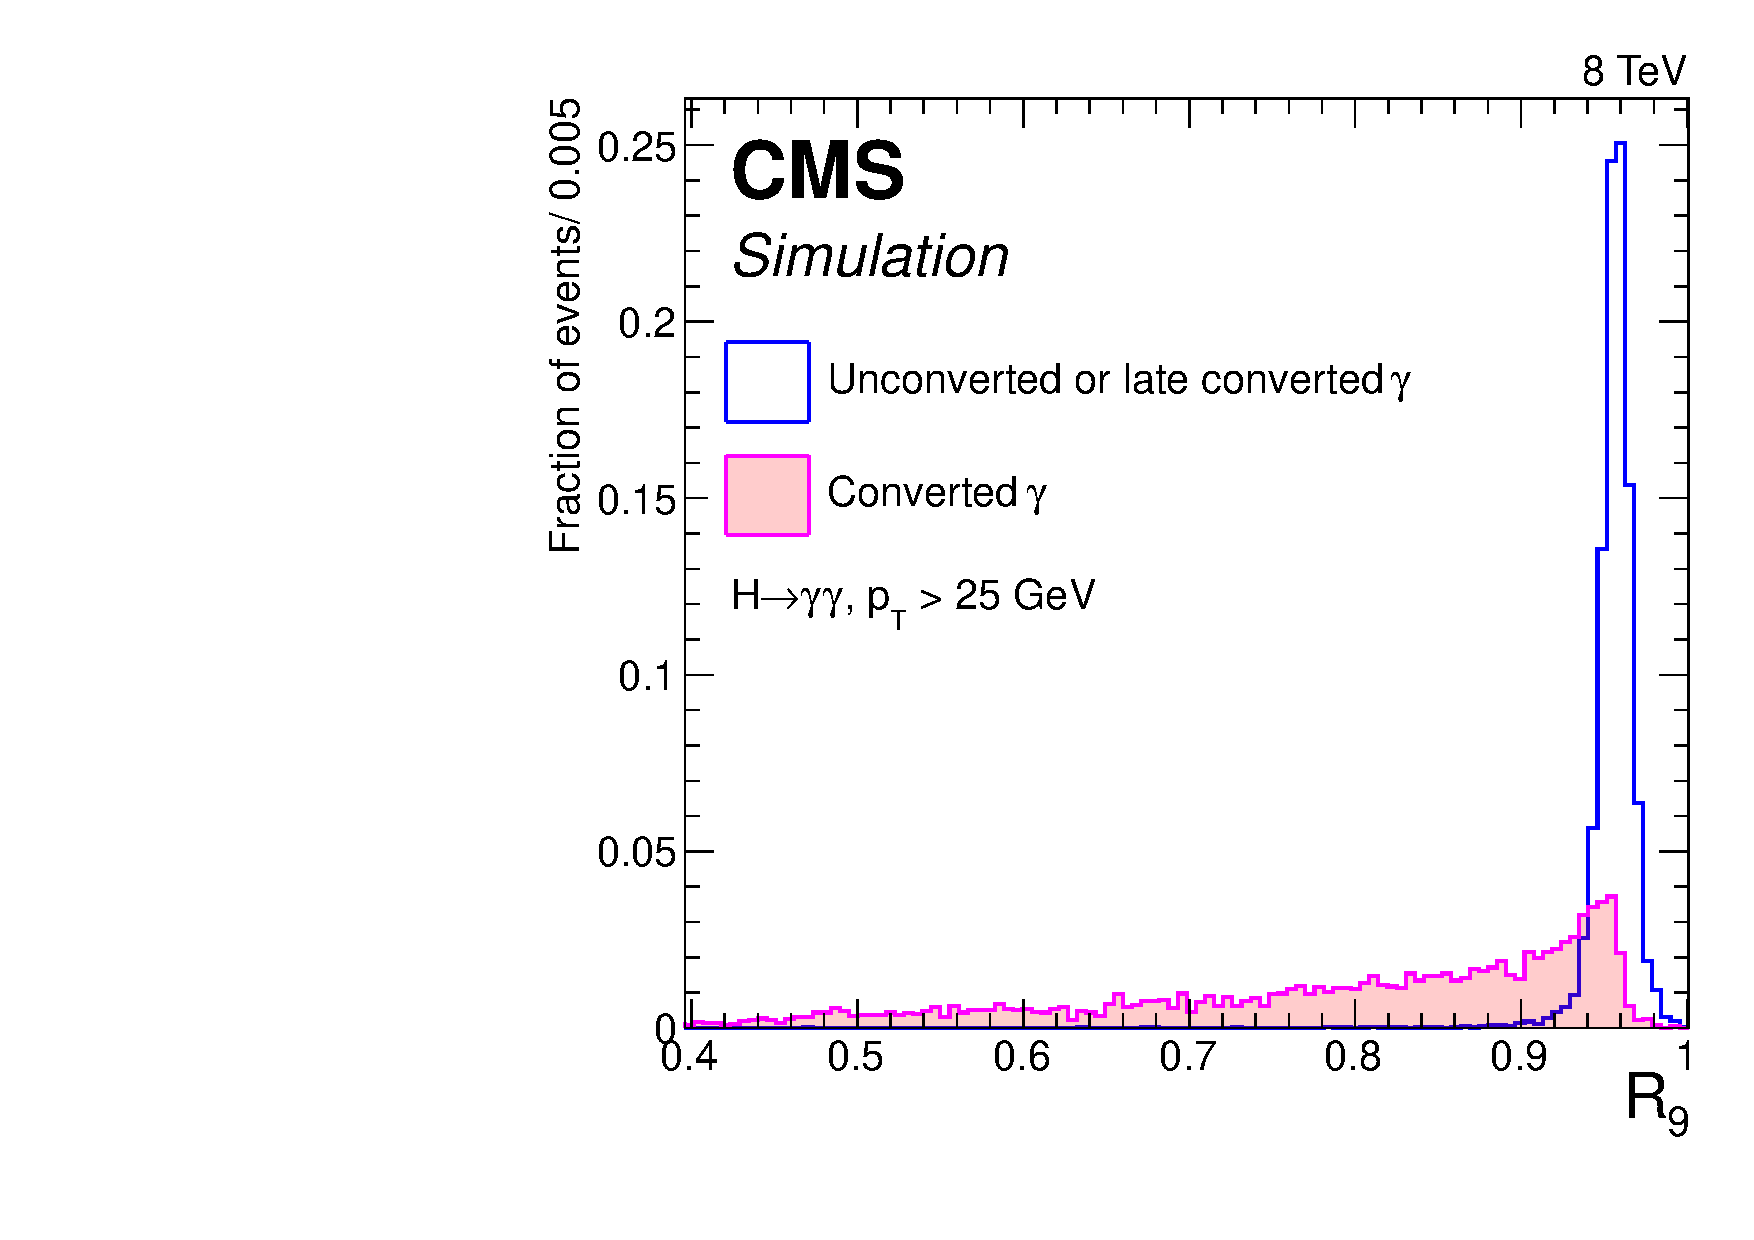
\includegraphics[width=0.50\textwidth]{figures/experiment/ObjectReconstruction/convUnconvR9Linear}
      \caption{Normalised distribution of the $R_9$ variable for converted and unconverted (or late converted) photons. Taken from~\cite{bib:CMS:PhotonIdentification_8TeV}}  
  \label{fig:PhotonR9}
\end{figure}
The energy spread is wider for converted photons than for unconverted photons.
Thus, the energy is estimated as the sum of energy deposits in the superclusters for converted photons ($R_9<0.94$ in the barrel and $R_9<0.94$ in the endcap region) and as the sum of energy deposits in the $5\times5$ crystal matrix for the unconverted photons.


\subsection{Reconstruction of muons}
\label{subsec:MuonReconstruction}
There are three different muon definitions at CMS~\cite{bib:CMS:muon_recoEff}: global muons, tracker muons, and standalone muons.
They all have in common that they require energy deposits in the muon system.
The reconstruction of each of the three muon types is explained in the following.
\begin{description}
\item \textbf{Standalone muons:} For the reconstruction of standalone muons, all reconstructed segments in the muon system are utilised. 
                                 Similar to the track reconstruction in the tracking system, Kalman filter techniques~\cite{bib:KalmanFilter_1987} are exploited to reconstruct muon trajectories in the muon chambers.
                                 A compatibility to the interaction point is imposed to reconstruct only muons produced at the LHC (no cosmic muons).
                                 Further details about the reconstruction of standalone muons can be found in~\cite{bib:StandaloneMuonReconstruction,bib:CMS:TDR_2006} 
\item \textbf{Tracker muons:} To reconstruct so-called tracker muons, all tracker tracks with a $\pt>0.5\gev$ and $p>2.5\gev$ are extrapolated to the muon system. 
                              If at least one muon segment is matched to a reconstructed track fulfilling certain quality criteria, the trajectory is considered as a tracker muon (see~\cite{bib:CMS:muon_recoEff} for more detailed information).
\item \textbf{Global muons:} For the reconstruction of global muons an outside-in approach is utilised. 
                             For each reconstructed standalone muon, the compatibility to the reconstructed tracks in the tracking system is checked. 
                             If compatible, a global muon track is reconstructed using Kalman filter techniques. 
                             For high-\pt muons, the momentum resolution can be increased this way compared to the momentum estimated using tracker information only~\cite{bib:CMS:muon_recoEff}.
\end{description}

\subsection{Reconstruction of electrons}
\label{subsec:ElectronReconstruction}
The reconstruction of electrons at the CMS experiment is based on a mixture of the particle-flow algorithm explained in Section~\ref{sec:PFalgorithm} and a standalone approach~\cite{bib:StandaloneElectronReconstruction}.
Thus, it is a very complex procedure and only the basic approach shall be explained here.
The reader is referred to~\cite{bib:CMS:elec_recoEff} for a complete description of the reconstruction procedure.

Electrons are identified using clustered energy deposits in the ECAL and reconstructed tracks in the tracker system. 
Both inputs are tested on compatibility and finally used to estimate the electron properties. 

The difficulty of the electron reconstruction lies in the possibly large energy losses due to bremsstrahlung.
This can change the direction of the electron significantly and lead to a reduced efficiency of the standard track reconstruction as well as a reduced efficiency of the association of ECAL clusters to the reconstructed track in the inner tracking system.
Therefore, an optimised track reconstruction for electrons is additionally performed in order to account for direction changes due to the radiation of photons.
Because the dedicated electron track reconstruction can be very time consuming, the seeding of tracker hits relies already on ECAL information to reduce the number of candidate tracks (ECAL-based seeding).

Therefore, the electron reconstruction proceeds in detail as follows.
First, ECAL clusters, so-called superclusters, are formed using a ``hybrid'' algorithm in the barrel region and a ``multi-$5\times 5$'' algorithm in the endcaps.
It is the same clustering used for photons (see Section~\ref{subsec:PhotonReconstruction} where the more information about these algorithms can be found).
Superclusters are used, since due to bremsstrahlung, the energy deposits by electrons are usually spread out over several crystals.
Additionally, so-called PF clusters are formed that add all neighbouring crystals to the above mentioned superclusters. 
Afterwards, the standard track reconstruction is performed which is able to reconstruct electron tracks when bremsstrahlung is negligible.
Very short reconstructed tracks or tracks with a bad $\chi^2$ are refitted using a so-called Gaussian sum filter (GSF)~\cite{bib:GSF_2003} to account for electrons with high radiative energy losses.
As mentioned above, these tracks use ECAL-based seeding to reduce the number of candidate tracks.  
To identify these refitted tracks as candidate electron tracks, a multivariate analysis is performed using tracker and ECAL information.
All ECAL PF clusters tangent to the electron track are added in order to capture the energy of bremsstrahlung photons.
Finally, track-cluster association criteria are applied in order to reduce misidentification while preserving a high reconstruction efficiency.
The association criteria rely on spatial distances between the superclusters and the tracker track for ECAL-seeded tracks (GSF tracks) and rely on multivariate techniques for the tracker-seeded (standard track reconstruction) electrons.

\subsection{Reconstruction of taus}
\label{subsec:TauReconstruction}
The tau reconstruction at CMS refers to the reconstruction of hadronically decaying taus (a fraction of around 65\% of taus decays hadronically).
Leptonically decaying taus can be identified through the reconstruction of the muon or the electron in the final state.
In the following a tau refers therefore to hadronically decaying taus only.
At CMS, the main algorithm used to identify and reconstruct taus is the so-called hadron plus strip algorithm (HPS)~\cite{bib:CMS:TauReconstruction_8TeV,bib:CMS:TauReconstruction_7TeV}, which is also used in this thesis.
The description of the tau reconstruction algorithm within this thesis follows~\cite{bib:CMS:TauReconstruction_8TeV}.

The HPS algorithm consists of two separate steps. 
First, reconstructed PF particles are combined in a way that they are compatible with any of the tau decay modes and the four-momentum of this combined object is estimated.
Second, multivariate techniques are used in order to discriminate the candidate taus against decays from gluon or quark jets and from muons and electrons. 
The HPS algorithm starts from reconstructed jets with a radius parameter of $R=0.5$ and $\pt>14\gev$ and $|\eta|<2.5$.

The successful identification of a tau requires the reconstruction of a neutral pion.
A neutral pion is present in most of the hadronic decays and decays into two photons with a probability of $\sim 99\%$. 
The photons in turn convert into electron pairs with a high probability inside the tracker volume.
Therefore, photons and electrons are clustered into strips in the $\eta-\phi$ plane in order to identify possible $\pi^0$.
The initial position of the strip equals the position of the seed electron or photon, \ie the photon or electron with the highest \pt not yet clustered into any strip.
The next-highest \pt electron/photon within a certain distance ($\eta \times \phi = 0.05 \times 0.20$) to the original strip is merged into the strip.
Afterwards, the strip position is recalculated and the step is repeated.
The clustering stops if no more electrons/photons are found.

After the reconstruction of the neutral pion, multiple decay mode hypotheses are tested by combining up to two clustered strips with one or three charged PF hadrons.
For all hypotheses, several restrictions on the invariant mass of the hadronically decaying tau are imposed.
Finally, the hypothesis fulfilling the invariant mass requirement and - in case this happens for more than one hypothesis - the one with the highest \pt tau is chosen.

Furthermore, for all taus in this thesis, the discriminators used for the reduction of jet, electron and muon contamination are required to be zero (see~\cite{bib:CMS:TauReconstruction_8TeV} for further details on the discriminators).

Finally, a loose isolation criterion is imposed, which is calculated by the pileup corrected scalar sum of the transverse momentum of all charged particles and photons with a \pt larger than 0.5\gev in a cone of $R=0.5$ around the tau.

\subsection{Reconstruction of missing transverse energy}
The particle-flow missing transverse energy, PF \met, in an event is defined as the negative vectorial sum of all particle-flow particles' \pt.
Thus - neglecting momentum mismeasurements - it refers to the transverse momentum of all only weakly interacting particles in the event.
In order to avoid negative effects from \eg tracker inefficiencies, non-linear calorimeter responses, etc., \met can be measured more precisely by correcting the transverse momentum of all jets contained in an event with the jet energy corrections (see Section~\ref{sec:JetReconstruction}).

For a more detailed explanation of \met as well as for information on the performance of the reconstruction, the reader is referred to~\cite{bib:CMS:METReconstruction}

\section{Event cleaning}
The two analyses described in this thesis are subject to an event cleaning procedure as recommended by the CMS collaboration~\cite{bib:CMS:EventCleaning}.
It refers to the application of several filters to remove events with detector signals not caused by particles from the hard interaction. 
In the following, the filters are listed and a short description will be given.
\begin{description} 
\item \textbf{HBHE noise filter:} This filter rejects anomalous HCAL noise in the barrel (HB) and in the endcap (HE). 
                                  The noise in the HCAL is mainly related to the hybrid photodiodes (HPD) and readout boxes (RBX). 
                                  It rejects events considering pulse shape information and anomalous high hit multiplicities in an HPD or RBX.
\item \textbf{CSC beam halo filter:} Particles contained in the beam halo can induce signals in the detector. 
                                     Therefore, events with a muon moving parallel to the beam are rejected.  
\item \textbf{HCAL laser event filter:} This filter provides a list of events, where the laser used for the HCAL calibration fired when a bunch crossing occurred. 
                                        Detector signals from the laser can be misinterpreted as particle signals and, therefore, these events are removed.
\item \textbf{ECAL dead cell filter:} Events with jets pointing towards a non-working ECAL cell are rejected. 
                                      This filter relies on information of the surrounding crystals as well as on ``trigger-primitive'' information.
\item \textbf{EE bad supercrystal filter:} In the ECAL endcap, two supercrystals were not working properly during the data taking period in 2012. 
                                           Therefore, events where at least one of the two crystals detected unnaturally high energy deposits are removed. 
\item \textbf{Tracking failure filter:} Sometimes, unnaturally high energy deposits are recorded in the calorimeters without corresponding tracks in the inner tracking system. 
                                        The reconstruction of tracks can fail, because of too many tracker seeds or because the hard interaction was too far away from the interaction point.
                                        This filter rejects therefore events, where less than 10\% of the energy in the event was measured by the tracker.  
\item \textbf{Scraping filter (data only):} When there are at least ten tracks in the event, at least 25\% of them need to be flagged as high-purity tracks as defined in~\cite{bib:CMS:Tracking_2010}.
\item \textbf{Tracking POG filter:} Events with aborted track reconstruction and/or strip tracker noise are rejected.
\end{description}



%%%%%%%%%%%%%%%%%%%%%%%%%%%%%%%%%%%%%%%%%%%%%%%%%%%%%%%%%%%%%%%%%%%%%%%%%%%%%%%%%%%%%%%%%%%%%%%%%%%%%%%%%%%%%%%%%%%%%%%%%%%%%%%%%%%%%%%%%%%%%%%%%%%%%%%%%%%%%%%%%%%%%%%%%%%%%%%%%%%%%%%%%%%%%%%%%%%%%%%%%%%%%%%%%%%%%%%%%%%%%%%%%%%
%%%%%%%%%%%%%%%%%%%%%%%%%%%%%%%%%%%%%%%%%%%%%%%%%%%%%%%%%%%%%%%%%%%%%%%%%%%%%%%%%%%%%%%%%%%%%%%%%%%%%%%%%%%%%%%%%%%%%%%%%%%%%%%%%%%%%%%%%%%%%%%%%%%%%%%%%%%%%%%%%%%%%%%%%%%%%%%%%%%%%%%%%%%%%%%%%%%%%%%%%%%%%%%%%%%%%%%%%%%%%%%%%%%
%%%%%%%%%%%%%%%%%%%%%%%%%%%%%%%%%%%%%%%%%%%%%%%%%%%%%%%%%%%%%%%%%%%%%%%%%%%%%%%%%%%%%%%%%%%%%%%%%%%%%%%%%%%%%%%%%%%%%%%%%%%%%%%%%%%%%%%%%%%%%%%%%%%%%%%%%%%%%%%%%%%%%%%%%%%%%%%%%%%%%%%%%%%%%%%%%%%%%%%%%%%%%%%%%%%%%%%%%%%%%%%%%%%
\FloatBarrier
\chapter{Simulation of events}
\label{ch:SimulationOfEvents}

A very important input for physics analyses at particle colliders is the use of simulated collision events.
They serve as a comparison to measured data and can give an estimation of the expected number of background and signal events for a given selection.
Furthermore, they are used to study event kinematics for Standard Model (SM) and beyond-SM processes.

The generation of simulated samples is done with the help of Monte Carlo (MC) methods (see \eg~\cite{bib:MC_Introduction}).
MC techniques are used to randomly sample points according to a specified probability distribution.
The underlying probability distributions for the event generation are the transition probabilities from the initial into all possible final states.

Besides the simulation of the hard interaction of the event, also the subsequent showering and hadronisation as well as the detector response needs to be simulated.
In the following sections, a short introduction into the various steps of event simulation is given.
For more information, the reader is referred to~\cite{bib:Matthias_Thesis}.\\

The first step of the generation of \pp-collision events consists of the simulation of the hard process, \ie the primary interaction of two partons of the two colliding protons.
Which types of partons are involved in the primary interaction is specified by so-called parton distribution functions (PDFs).
They describe the probability of a parton (up-quarks, down-quarks, gluons, sea quarks) to carry a certain energy fraction of the proton and thus define the probability for each parton to take part in the hard interaction process.
%In this thesis, all simulated samples are generated with the PDFs provided by the \cteq group~\cite{Pumplin:2002vw} 

After the simulation of the hard interaction between the selected partons, the showering and hadronisation of the particles is simulated.
Throughout this thesis, the matrix element generator \madgraph~\cite{bib:Madgraph_2014} plus the event generator \pythia~\cite{bib:Pyhtia6_2006} or the event generator \pythia only are used.
Since \madgraph only provides the generation of matrix elements, the subsequent showering and hadronisation is done by \pythia.
For this task, particles produced in the hard interaction are matched to the particles produced in the showers in order to avoid a double-counting of emissions in multijet processes.
Since \madgraph is responsible for the simulation of well separated partons whereas \pythia is designed for simulating the soft and collinear showers, the event is rejected if a parton from the matrix element generator cannot be matched within a certain distance $\Delta R$ to any of the simulated showers (MLM matching scheme~\cite{bib:MLM_matching}).
The showers are clustered with the \kt method (see Section~\ref{sec:JetReconstruction}).
Additionally, events are rejected if there are more showers than partons in the event.

The formation of colour neutral particles, called hadronisation, and the subsequent decay of unstable particles is simulated with \pythia for all samples used in this thesis.
A visualisation of the various steps performed for the generation of events is shown in Fig.~\ref{fig:MCsimulation}. 
%\begin{figure}[!t]
%  \centering
%      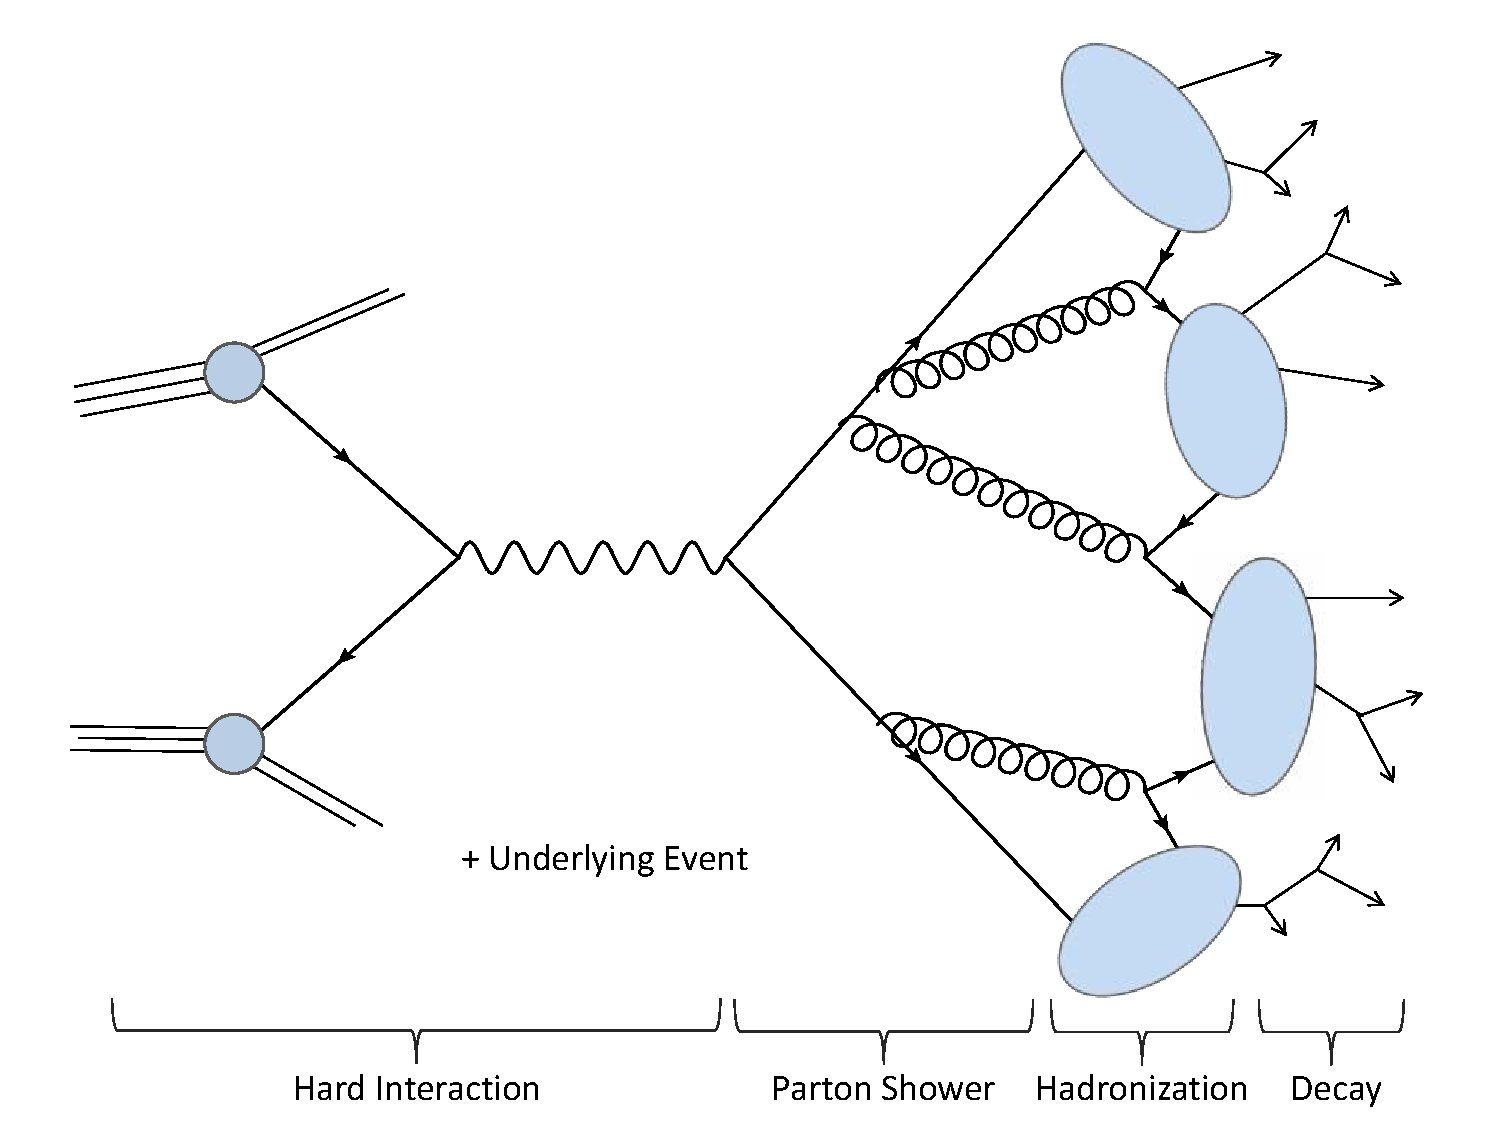
\includegraphics[width=0.60\textwidth]{figures/experiment/Simulation/MCGeneration}
%  \caption{Visualisation of the various steps performed in the simulation of events. Taken from~\cite{bib:Kristin_Thesis}.}  
%  \label{fig:MCsimulation}
%\end{figure}

In order to account for signals caused by the interaction of the non-primary partons of the interacting protons - called the underlying event (UE) -  various models (tunes) are exploited.
They rely on the measured signals in data in proton collisions without any hard interaction.
Detector signals caused by additional interactions (pileup interactions) during a bunch-crossing, are also mixed into every simulated sample.

Finally, the interaction of the traversing particles with the detector material as well as the response and the readout electronics is simulated with \geant~\cite{bib:Geant4_2003,bib:Geant4_2006} throughout this thesis.


